\chapter{Livrables numériques}
\label{annexe:livrables-numeriques}

Dans le cadre du master 2 \enquote{Technologies numériques appliquées à l'histoire}, le stage comprend obligatoirement la réalisation d'un livrable technique, évalué avec le stage, le mémoire et la soutenance. Ce livrable correspond à une production concrète mettant en œuvre les compétences acquises pendant la formation : prototype d'application ou d'interface web, code source, script de traitement, jeu de données ou chaîne de traitement.\footnote{École nationale des chartes -- PSL, \enquote{Appel à stages et alternances pour le master Technologies numériques appliquées à l'histoire}, \url{https://www.chartes.psl.eu/appel-stages-et-alternances-pour-le-master-technologies-numeriques-appliquees-lhistoire}, consulté le 30 août 2026.}

Deux livrables numériques accompagnent ce mémoire : le prototype du mini-site des archives historiques de médecine et le dépôt consacré à l'analyse des exports EAD du module Archives de Flora. Le premier matérialise les propositions d'organisation, de consultation et de valorisation formulées pendant le stage. Le second rassemble les jeux de test, les exports XML, les scripts Python et les résultats de validation ayant servi à évaluer l'interopérabilité de Flora.

\clearpage
\section{Prototype du mini-site des archives historiques de médecine}
\label{annexe:prototype-mini-site}

\subsection{Accès et statut}

Le code source du prototype est déposé sur GitHub :

\begin{center}
	\url{https://github.com/CMartinArchives/prototype-minisite-medecine}
\end{center}

Une version statique est temporairement déployée avec GitHub Pages :

\begin{center}
	\url{https://cmartinarchives.github.io/prototype-minisite-medecine/}
\end{center}

Ces accès resteront publics pendant l'évaluation du mémoire, puis passeront en privé dans l'attente de la validation institutionnelle et de la publication du mini-site WordPress. Cette restriction tient également aux droits associés aux reproductions numériques.

Le prototype est un démonstrateur fonctionnel destiné à représenter une organisation possible du mini-site, à recueillir les besoins de la Mission Archives historiques et à fournir un support aux services et aux instances chargés de valider le projet.

Les fonctions retenues pourront être transposées dans le modèle WordPress de l'Université, dans les limites de ses composants.

\subsection{Arborescence du dépôt}

\begin{minipage}{\textwidth}
	\footnotesize
	\begin{verbatim}
		.
		|-- index.html
		|-- pages/
		|   |-- consultation.html
		|   |-- expositions.html
		|   |-- instruments-recherche.html
		|   `-- musee-archives.html
		|-- assets/
		|   |-- css/
		|   |   `-- site.css
		|   |-- js/
		|   |   |-- site.js
		|   |   `-- musee-archives.js
		|   `-- images/
		|       |-- accueil/
		|       |-- expositions/
		|       |-- identite/
		|       |-- instruments/
		|       `-- musee-archives/
		`-- documents/instruments-recherche/
				|-- 1fimed.pdf
				|-- 1med.pdf
				`-- 2med.pdf
	\end{verbatim}
\end{minipage}

\subsection{Périmètre fonctionnel}

Le prototype comprend cinq pages :

\begin{itemize}
	\item l'accueil, consacré à la Mission Archives historiques et à la présentation générale des fonds ;
	\item les fonds et instruments de recherche ;
	\item les expositions et projets de valorisation ;
	\item les informations de consultation et l'aide à la recherche ;
	\item la restitution numérique du \enquote{musée des archives}.
\end{itemize}

La page documentaire réunit le fonds ancien et les fonds modernes et contemporains publics et privés. Ces derniers étaient répartis sur trois pages dans le test WordPress ; leur regroupement facilite ici le parcours de consultation.

Seuls les instruments 1MED, 2MED et 1FiMED sont joints au dépôt, car ils avaient déjà fait l'objet d'une publication en ligne. Les instruments internes ou inédits ne sont pas diffusés.

Les plans de classement étaient encore en cours d'élaboration au moment du mémoire. Leur intégration ultérieure pourrait prendre la forme de deux arborescences présentant l'ensemble des fonds publics et privés, y compris ceux dépourvus d'instrument publié. Des liens associés à des identifiants de fragments HTML renverraient vers les notices disponibles. La représentation du fonds général ne serait ainsi pas limitée aux seuls ensembles déjà décrits et publiés.

La page de consultation présente l'organisation des archives en fonds, la lecture d'un inventaire, le repérage d'une cote et les informations nécessaires à une demande de consultation.

\subsection{Restitution du musée des archives}
\label{annexe:musee-archives}

La visionneuse restitue les vingt-deux documents sélectionnés par Joseph Calmette au début du XX\textsuperscript{e} siècle. Pour chaque pièce, elle affiche la cote, la date, une courte notice et une ou plusieurs reproductions.

Une liste latérale, des commandes précédent et suivant et des boutons de changement de vue assurent la navigation. Les images peuvent être agrandies, zoomées ou ouvertes séparément.

Les numérisations ont été réalisées par Clara Martin pendant le stage. Certains parchemins de la série B ont été reproduits dans leur état matériel actuel et apparaissent encore pliés. Leur mise à plat et leur restauration doivent être effectuées par les ateliers du \gls{scdi}. Leur mise à disposition temporaire ne constitue pas une autorisation de réutilisation.

\subsection{Architecture technique}

Le prototype est un site statique sans back-end, base de données, dépendance externe ni chaîne de compilation. Les pages utilisent une structure HTML5 sémantique, des chemins relatifs et des identifiants de fragments pour la navigation interne.

La feuille \texttt{site.css} centralise la présentation. La mise en page repose sur CSS Grid, Flexbox et des requêtes \texttt{@media} pour l'affichage adaptatif. Les fenêtres modales et les états actifs sont contrôlés par des classes CSS.

Le fichier \texttt{site.js}, écrit en JavaScript natif, utilise des écouteurs d'événements, des attributs \texttt{data-*} et des transformations CSS pour gérer les modales, le zoom et le déplacement des images.

Le fichier \texttt{musee-archives.js} stocke les notices dans un tableau d'objets. Il génère dynamiquement la liste des documents et actualise le DOM selon l'index du document et de la vue sélectionnés. Il assure également la navigation cyclique, les commandes au clavier et le zoom.

Git assure le versionnement du code. GitHub héberge le dépôt et GitHub Pages sert les ressources statiques depuis la branche principale.

\subsection{Limites}

L'absence de CMS impose de modifier directement les fichiers HTML ou JavaScript. Le prototype ne comporte ni moteur de recherche, ni formulaire actif, ni interrogation de données structurées.

La visionneuse ne prend pas en charge les fonctions avancées d'IIIF et de Mirador, telles que les manifestes normalisés, le chargement par régions ou la comparaison de plusieurs documents.

Les plans de classement, les coordonnées, l'accessibilité, les droits de diffusion et les modalités d'intégration dans WordPress devront être validés avant la réalisation institutionnelle.

\clearpage
\section{Analyse de l'export EAD du module Archives de Flora}
\label{annexe:analyse-flora}

\subsection{Accès, contenu et périmètre}

Les fichiers ayant servi à l'évaluation sont documentés dans le dépôt GitHub suivant :

\begin{center}
	\url{https://github.com/CMartinArchives/flora-ead-analysis}
\end{center}

Le dépôt restera public pendant l'évaluation du mémoire, puis passera en accès privé. Il contient des jeux de données fictifs, six exports XML, leurs résultats de validation, un script d'analyse et un script de correction expérimentale.

Les exports ont été produits depuis une instance de préproduction de Flora mise à disposition de l'Université dans le cadre du déploiement du logiciel. Aucune donnée archivistique réelle ou confidentielle n'est diffusée, mais ces fichiers techniques n'ont pas vocation à rester accessibles au-delà de l'évaluation.

Les résultats correspondent à la configuration testée à l'été 2026. Ils ne constituent pas une évaluation générale de Flora et ne préjugent pas des corrections, paramétrages ou évolutions ultérieures de son export EAD.

\subsection{Arborescence du dépôt}

\begin{minipage}{\textwidth}
	\footnotesize
	\begin{verbatim}
		.
		|-- analyser_exports.py
		|-- corriger_export_minimal.py
		|-- requirements.txt
		|-- dtd/
		|   `-- ead.dtd
		|-- exports/
		|   |-- 01_export_minimal_a_plat.xml
		|   |-- 02_export_a_plat_versement_enrichi.xml
		|   |-- 03_export_a_plat_article_enrichi.xml
		|   |-- 04_export_hierarchique_deux_niveaux.xml
		|   |-- 05_export_hierarchique_trois_niveaux.xml
		|   `-- 06_export_hierarchique_deux_branches.xml
		`-- rapports/
		|-- analyse.json
		`-- 01_export_minimal_a_plat_corrige.xml
	\end{verbatim}
\end{minipage}

Le fichier \texttt{requirements.txt} indique la dépendance à la bibliothèque Python \texttt{lxml}. Le dossier \texttt{dtd} contient la DTD EAD 2002 utilisée pour la validation. Le dossier \texttt{exports} rassemble les fichiers produits par Flora, tandis que le dossier \texttt{rapports} contient le rapport JSON et l'export minimal corrigé.

\subsection{Objectif et protocole}

L'expérimentation visait à déterminer si les descriptions saisies ou importées dans Flora pouvaient être exportées en EAD 2002 et réutilisées dans Calames ou FranceArchives.

Les tests ont porté sur :

\begin{itemize}
	\item une structure minimale à plat composée d'un versement et de trois articles ;
	\item deux structures à plat comportant des descriptions enrichies ;
	\item une hiérarchie composée d'un article et de deux dossiers ;
	\item une hiérarchie à trois niveaux : article, dossier et sous-dossier ;
	\item deux branches indépendantes de type article--dossier ;
	\item l'export simultané de plusieurs versements.
\end{itemize}

Les fichiers XML ont été validés contre la DTD EAD 2002. Le script \texttt{analyser\_exports.py} contrôle également leur bien-formation, le nombre de composants \texttt{<c>}, les identifiants répétés et la position des unités dans l'arborescence. Les résultats sont enregistrés dans un rapport JSON.

\subsection{Principaux résultats}

Le modèle interne de Flora permet de décrire plusieurs niveaux archivistiques et de les relier par des relations parent--enfant. L'export mobilise notamment les éléments EAD \texttt{<origination>}, \texttt{<unitdate>}, \texttt{<scopecontent>}, \texttt{<physdesc>} et \texttt{<bibliography>}.

Aucun des six fichiers contrôlés ne valide cependant directement contre la DTD EAD 2002. Le fichier minimal produit vingt-neuf erreurs, principalement dues :

\begin{itemize}
	\item à l'emploi d'éléments absents de la DTD ;
	\item à des modèles de contenu non respectés ;
	\item à l'emploi de \texttt{<unititle>} au lieu de \texttt{<unittitle>} ;
	\item à des blocs \texttt{<did>} incomplets.
\end{itemize}

Les exports à plat conservent un composant et un identifiant par unité. Dans les tests hiérarchiques, chaque unité enfant apparaît cependant comme composant autonome, puis de nouveau sous son parent. Le nombre de répétitions augmente avec la profondeur : dans l'essai à trois niveaux, le dossier est exporté deux fois et le sous-dossier trois fois.

L'export simultané de plusieurs versements a par ailleurs produit une archive ZIP vide de 22 octets dans l'instance testée.

\subsection{Correction expérimentale}

Le script \texttt{corriger\_export\_minimal.py} vérifie si les erreurs régulières du premier fichier peuvent être corrigées automatiquement. Il réalise :

\begin{itemize}
	\item le remplacement de \texttt{<unititle>} par \texttt{<unittitle>} ;
	\item le retrait des enveloppes non déclarées en conservant leur contenu ;
	\item la restructuration des éléments exigeant un contenu balisé ;
	\item la correction des blocs \texttt{<did>} incomplets.
\end{itemize}

Le fichier transformé valide contre la DTD EAD 2002. Le script constitue néanmoins une preuve de faisabilité limitée au fichier minimal : il ne couvre pas tous les champs des descriptions enrichies et ne reconstruit pas les hiérarchies dupliquées.

\subsection{Conclusion}

Dans la configuration étudiée, aucun des exports EAD produits par Flora n'était directement exploitable dans Calames ou FranceArchives. La correction automatisée du fichier minimal à plat constitue uniquement une preuve de faisabilité pour certaines erreurs syntaxiques ; elle ne traite ni les descriptions enrichies ni la duplication des unités dans les hiérarchies.

L'export EAD de Flora n'a donc pas été retenu pour la production ou le transfert des instruments de recherche. Cette fonction a été orientée vers des outils travaillant directement en EAD, notamment SimplEAD et Calames, tandis que Flora restait envisagé pour d'autres usages de gestion, de recherche et de diffusion.

\chapter{Proposition de modélisation en \gls{cidoccrm} autour de François Rabelais}
\label{annexe:rabelais-cidoccrm}

Le schéma suivant propose une modélisation partielle, fondée sur le \gls{cidoccrm}, de relations documentaires mises en évidence dans la série consacrée à François Rabelais sur \emph{Ex Bibliotheca}. Il ne vise ni à représenter exhaustivement le corpus ni à proposer un modèle de données destiné à l'Université de Montpellier, mais à éprouver, sur un ensemble restreint, la possibilité de relier une personne, des activités universitaires, les informations qui les attestent et leurs supports matériels conservés aux archives historiques et à la bibliothèque universitaire historique de médecine.

La modélisation distingue les objets physiques des contenus informationnels qu'ils portent. François Rabelais est représenté comme une instance de \emph{E21 Person} ; la collation de son doctorat et son enseignement comme des instances de \emph{E7 Activity} ; les périodes correspondantes comme des instances de \emph{E52 Time-Span}. Les registres S~5 et S~4, objets matériels conservés aux archives historiques, relèvent de \emph{E22 Human-Made Object}, tandis que les informations qu'ils portent sur le doctorat et l'enseignement sont représentées comme des instances de \emph{E31 Document}. Cette distinction permet d'exprimer la relation entre le support et son contenu par \emph{P128 carries}, puis la fonction documentaire de ce contenu par \emph{P70 documents}.

La même logique s'applique à la ressource bibliographique : l'exemplaire J~346 est représenté dans sa matérialité comme une instance de \emph{E22 Human-Made Object}, tandis que les \emph{Pronostics} d'Hippocrate constituent une instance de \emph{E33 Linguistic Object} portée par cet exemplaire. L'activité d'enseignement est reliée à ce texte par \emph{P16 used specific object}. Ces choix constituent une proposition expérimentale qui pourrait être affinée selon le niveau de granularité retenu et les informations disponibles dans les sources.

\begin{landscape}
	\begin{figure}[p]
		\centering
		
		\rotatebox{180}{%
			\begin{minipage}{\linewidth}
				\centering
				
				\begin{tikzpicture}[
					x=1cm,
					y=1cm,
					>=Stealth,
					instance/.style={
						draw,
						rounded corners,
						align=center,
						text width=3.8cm,
						minimum height=1.1cm
					},
					contenu/.style={
						draw,
						align=center,
						text width=4cm,
						minimum height=1.15cm
					},
					support/.style={
						draw,
						rounded corners,
						align=center,
						text width=4.1cm,
						minimum height=1.2cm
					},
					temps/.style={
						draw,
						rounded corners,
						align=center,
						text width=3cm,
						minimum height=0.9cm
					},
					relation/.style={
						->,
						thick
					},
					etiquette/.style={
						fill=white,
						inner sep=2pt,
						align=center,
						font=\small
					}
					]
					
					% ============================================================
					% PERSONNE
					% ============================================================
					
					\node[instance] (rabelais) at (-10,2.8)
					{\textbf{François Rabelais}\\
						{\scriptsize\itshape E21 Person}};
					
					% ============================================================
					% ACTIVITÉS
					% ============================================================
					
					\node[instance] (doctorat) at (-4.5,5.2)
					{\textbf{Collation du doctorat}\\
						de François Rabelais\\
						{\scriptsize\itshape E7 Activity}};
					
					\node[instance] (enseignement) at (-4.5,0.4)
					{\textbf{Enseignement des}\\
						\emph{Pronostics} d'Hippocrate\\
						{\scriptsize\itshape E7 Activity}};
					
					% ============================================================
					% PÉRIODES
					% ============================================================
					
					\node[temps] (tempsdoctorat) at (-0.5,7.5)
					{\textbf{22 mai 1537}\\
						{\scriptsize\itshape E52 Time-Span}};
					
					\node[temps] (tempsenseignement) at (-0.5,2.7)
					{\textbf{1537--1538}\\
						{\scriptsize\itshape E52 Time-Span}};
					
					% ============================================================
					% CONTENUS DOCUMENTAIRES DES ARCHIVES
					% ============================================================
					
					\node[contenu] (docdoctorat) at (4.2,5.2)
					{\textbf{Mention de la collation}\\
						\textbf{du doctorat}\\
						S~5, fol.~33\\
						{\scriptsize\itshape E31 Document}};
					
					\node[contenu] (docenseignement) at (4.2,0.4)
					{\textbf{Mention de l'enseignement}\\
						\textbf{des \emph{Pronostics}}\\
						S~4, fol.~36\\
						{\scriptsize\itshape E31 Document}};
					
					% ============================================================
					% SUPPORTS MATÉRIELS DES ARCHIVES
					% ============================================================
					
					\node[support] (s5) at (10,5.2)
					{\textbf{Registre des actes}\\
						S~5\\
						Archives historiques\\
						{\scriptsize\itshape E22 Human-Made Object}};
					
					\node[support] (s4) at (10,0.4)
					{\textbf{Registre des leçons}\\
						S~4\\
						Archives historiques\\
						{\scriptsize\itshape E22 Human-Made Object}};
					
					% ============================================================
					% TEXTE ET EXEMPLAIRE BIBLIOGRAPHIQUE
					% ============================================================
					
					\node[contenu] (pronostics) at (-1.5,-4.2)
					{\textbf{\emph{Pronostics}}\\
						Hippocrate\\
						{\scriptsize\itshape E33 Linguistic Object}};
					
					\node[support] (j346) at (6,-4.2)
					{\textbf{\emph{Hippocratis ac Galeni libri aliquot}}\\
						Lyon, 1532 --- J~346\\
						Bibliothèque universitaire historique de médecine\\
						{\scriptsize\itshape E22 Human-Made Object}};
					
					% ============================================================
					% ACTIVITÉS -> PERSONNE
					% ============================================================
					
					% Rabelais participe à la collation institutionnelle
					% de son doctorat.
					
					\draw[relation]
					(doctorat.west) --
					node[etiquette, sloped, above]
					{\textbf{P11} had participant}
					(rabelais.north east);
					
					% Rabelais accomplit l'activité d'enseignement.
					
					\draw[relation]
					(enseignement.west) --
					node[etiquette, sloped, below]
					{\textbf{P14} carried out by}
					(rabelais.south east);
					
					% ============================================================
					% ACTIVITÉS -> PÉRIODES
					% ============================================================
					
					\draw[relation]
					(doctorat.north east) --
					node[etiquette, sloped, above]
					{\textbf{P4} has time-span}
					(tempsdoctorat.south west);
					
					\draw[relation]
					(enseignement.north east) --
					node[etiquette, sloped, above]
					{\textbf{P4} has time-span}
					(tempsenseignement.south west);
					
					% ============================================================
					% CONTENUS DOCUMENTAIRES -> ACTIVITÉS
					% ============================================================
					
					% P70 relie directement le document à l'activité
					% qu'il documente.
					
					\draw[relation]
					(docdoctorat.west) --
					node[etiquette, above]
					{\textbf{P70} documents}
					(doctorat.east);
					
					\draw[relation]
					(docenseignement.west) --
					node[etiquette, above]
					{\textbf{P70} documents}
					(enseignement.east);
					
					% ============================================================
					% SUPPORTS D'ARCHIVES -> CONTENUS DOCUMENTAIRES
					% ============================================================
					
					% Le registre matériel porte le contenu documentaire.
					
					\draw[relation]
					(s5.west) --
					node[etiquette, above]
					{\textbf{P128} carries}
					(docdoctorat.east);
					
					\draw[relation]
					(s4.west) --
					node[etiquette, above]
					{\textbf{P128} carries}
					(docenseignement.east);
					
					% ============================================================
					% ACTIVITÉ D'ENSEIGNEMENT -> TEXTE UTILISÉ
					% ============================================================
					
					\draw[relation]
					(enseignement.south) --
					node[etiquette, left]
					{\textbf{P16} used specific object}
					(pronostics.north);
					
					% ============================================================
					% EXEMPLAIRE BIBLIOGRAPHIQUE -> TEXTE
					% ============================================================
					
					\draw[relation]
					(j346.west) --
					node[etiquette, above]
					{\textbf{P128} carries}
					(pronostics.east);
					
				\end{tikzpicture}
				
				\captionof{figure}
				[Proposition de modélisation en CIDOC CRM autour de François Rabelais]
				{Proposition expérimentale de modélisation en \gls{cidoccrm} de relations entre François Rabelais, ses activités universitaires, les contenus documentaires qui les attestent et leurs supports matériels conservés aux archives historiques et à la bibliothèque universitaire historique de médecine. Les classes et propriétés sont empruntées au \gls{cidoccrm} 7.1.3 ; leur application au corpus constitue une proposition de modélisation et non un modèle adopté par l'Université de Montpellier.}
				
				\label{fig:rabelais-cidoccrm}
				
			\end{minipage}%
		}
		
	\end{figure}
\end{landscape}

\chapter{Reproductions de documents conservés aux archives historiques de la Faculté de médecine de Montpellier}
\label{annexe:reproductions-ahfm}

Les reproductions réunies dans cette annexe ont été réalisées au cours
du stage à partir de documents conservés aux archives historiques de la
Faculté de médecine de Montpellier. Elles complètent les analyses du
mémoire en donnant accès à plusieurs pièces directement mobilisées dans
l'étude de la constitution et du traitement des fonds.

\begin{figure}[p]
	\centering
	
	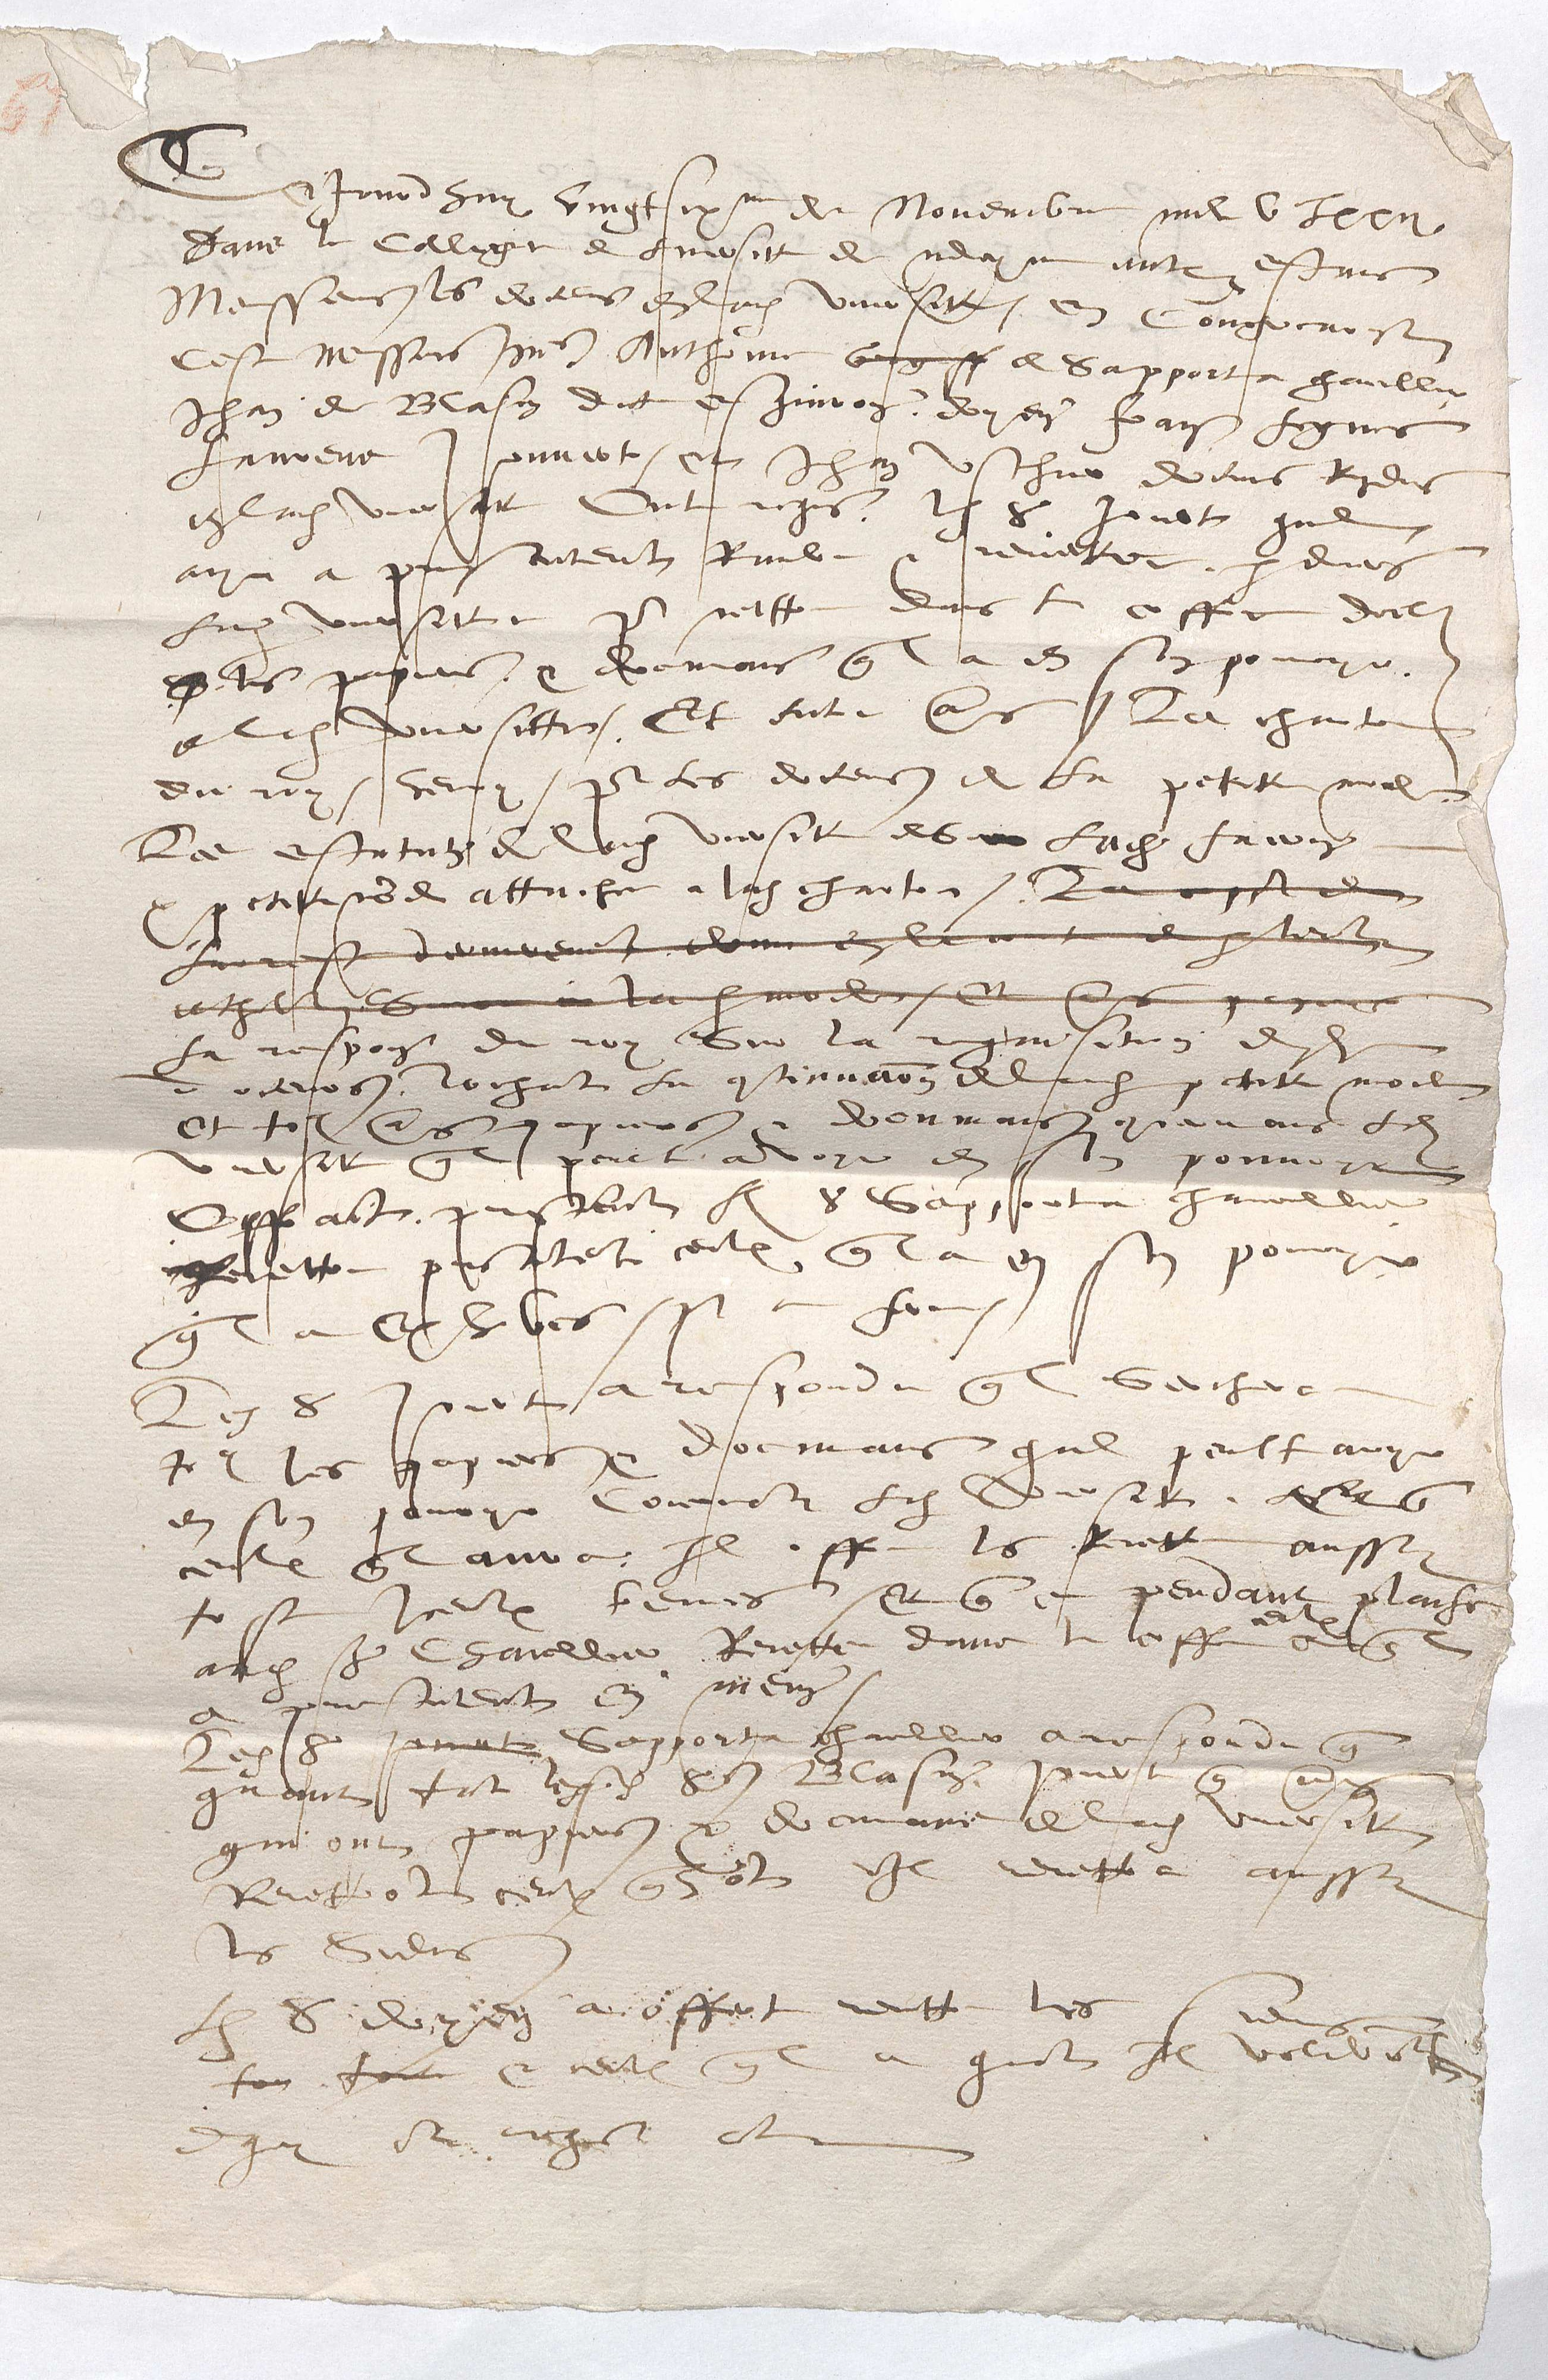
\includegraphics[
	width=\textwidth,
	height=0.65\textheight,
	keepaspectratio
	]{images/C17_01.jpg}
	
	\vspace{0.6em}
	
	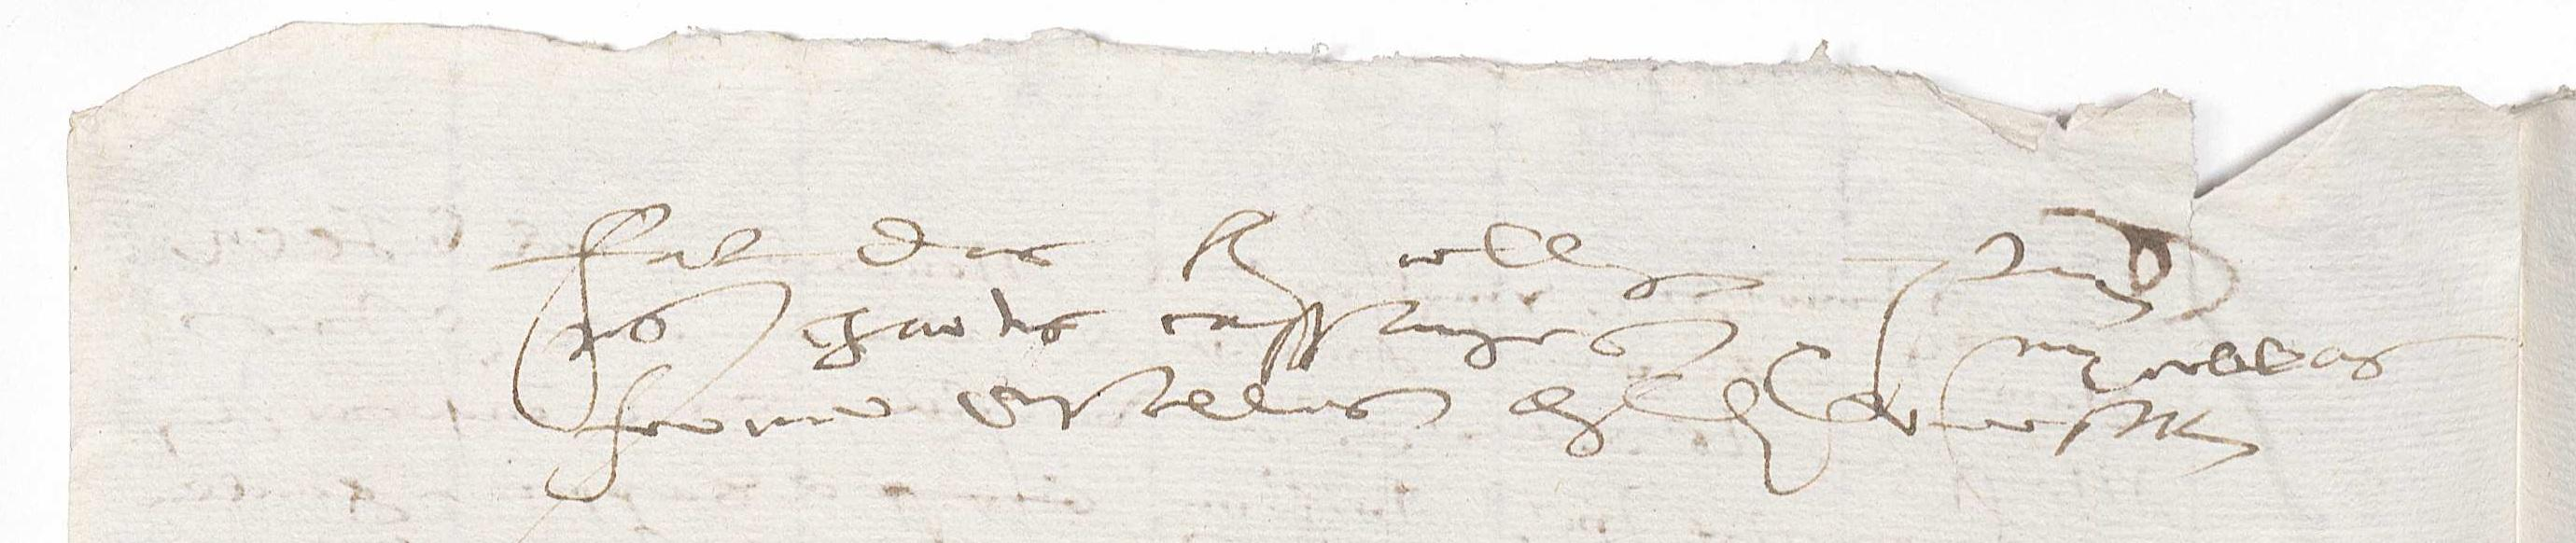
\includegraphics[
	width=\textwidth,
	height=0.12\textheight,
	keepaspectratio
	]{images/C17_02.jpg}
	
	\caption[Délibération demandant à Laurent Joubert de remettre des papiers de l'Université]
	{\enquote{Délibération en vertu de laquelle Laurent Joubert est invité à remettre certains papiers de l'Université qui sont entre ses mains}, 26 novembre 1572, recto et détail du verso recadré sur le passage final, Montpellier, Archives historiques de la Faculté de médecine, C~17. Numérisation : Clara Martin.}
	\label{fig:c17}
\end{figure}

\begin{figure}[p]
	\centering
	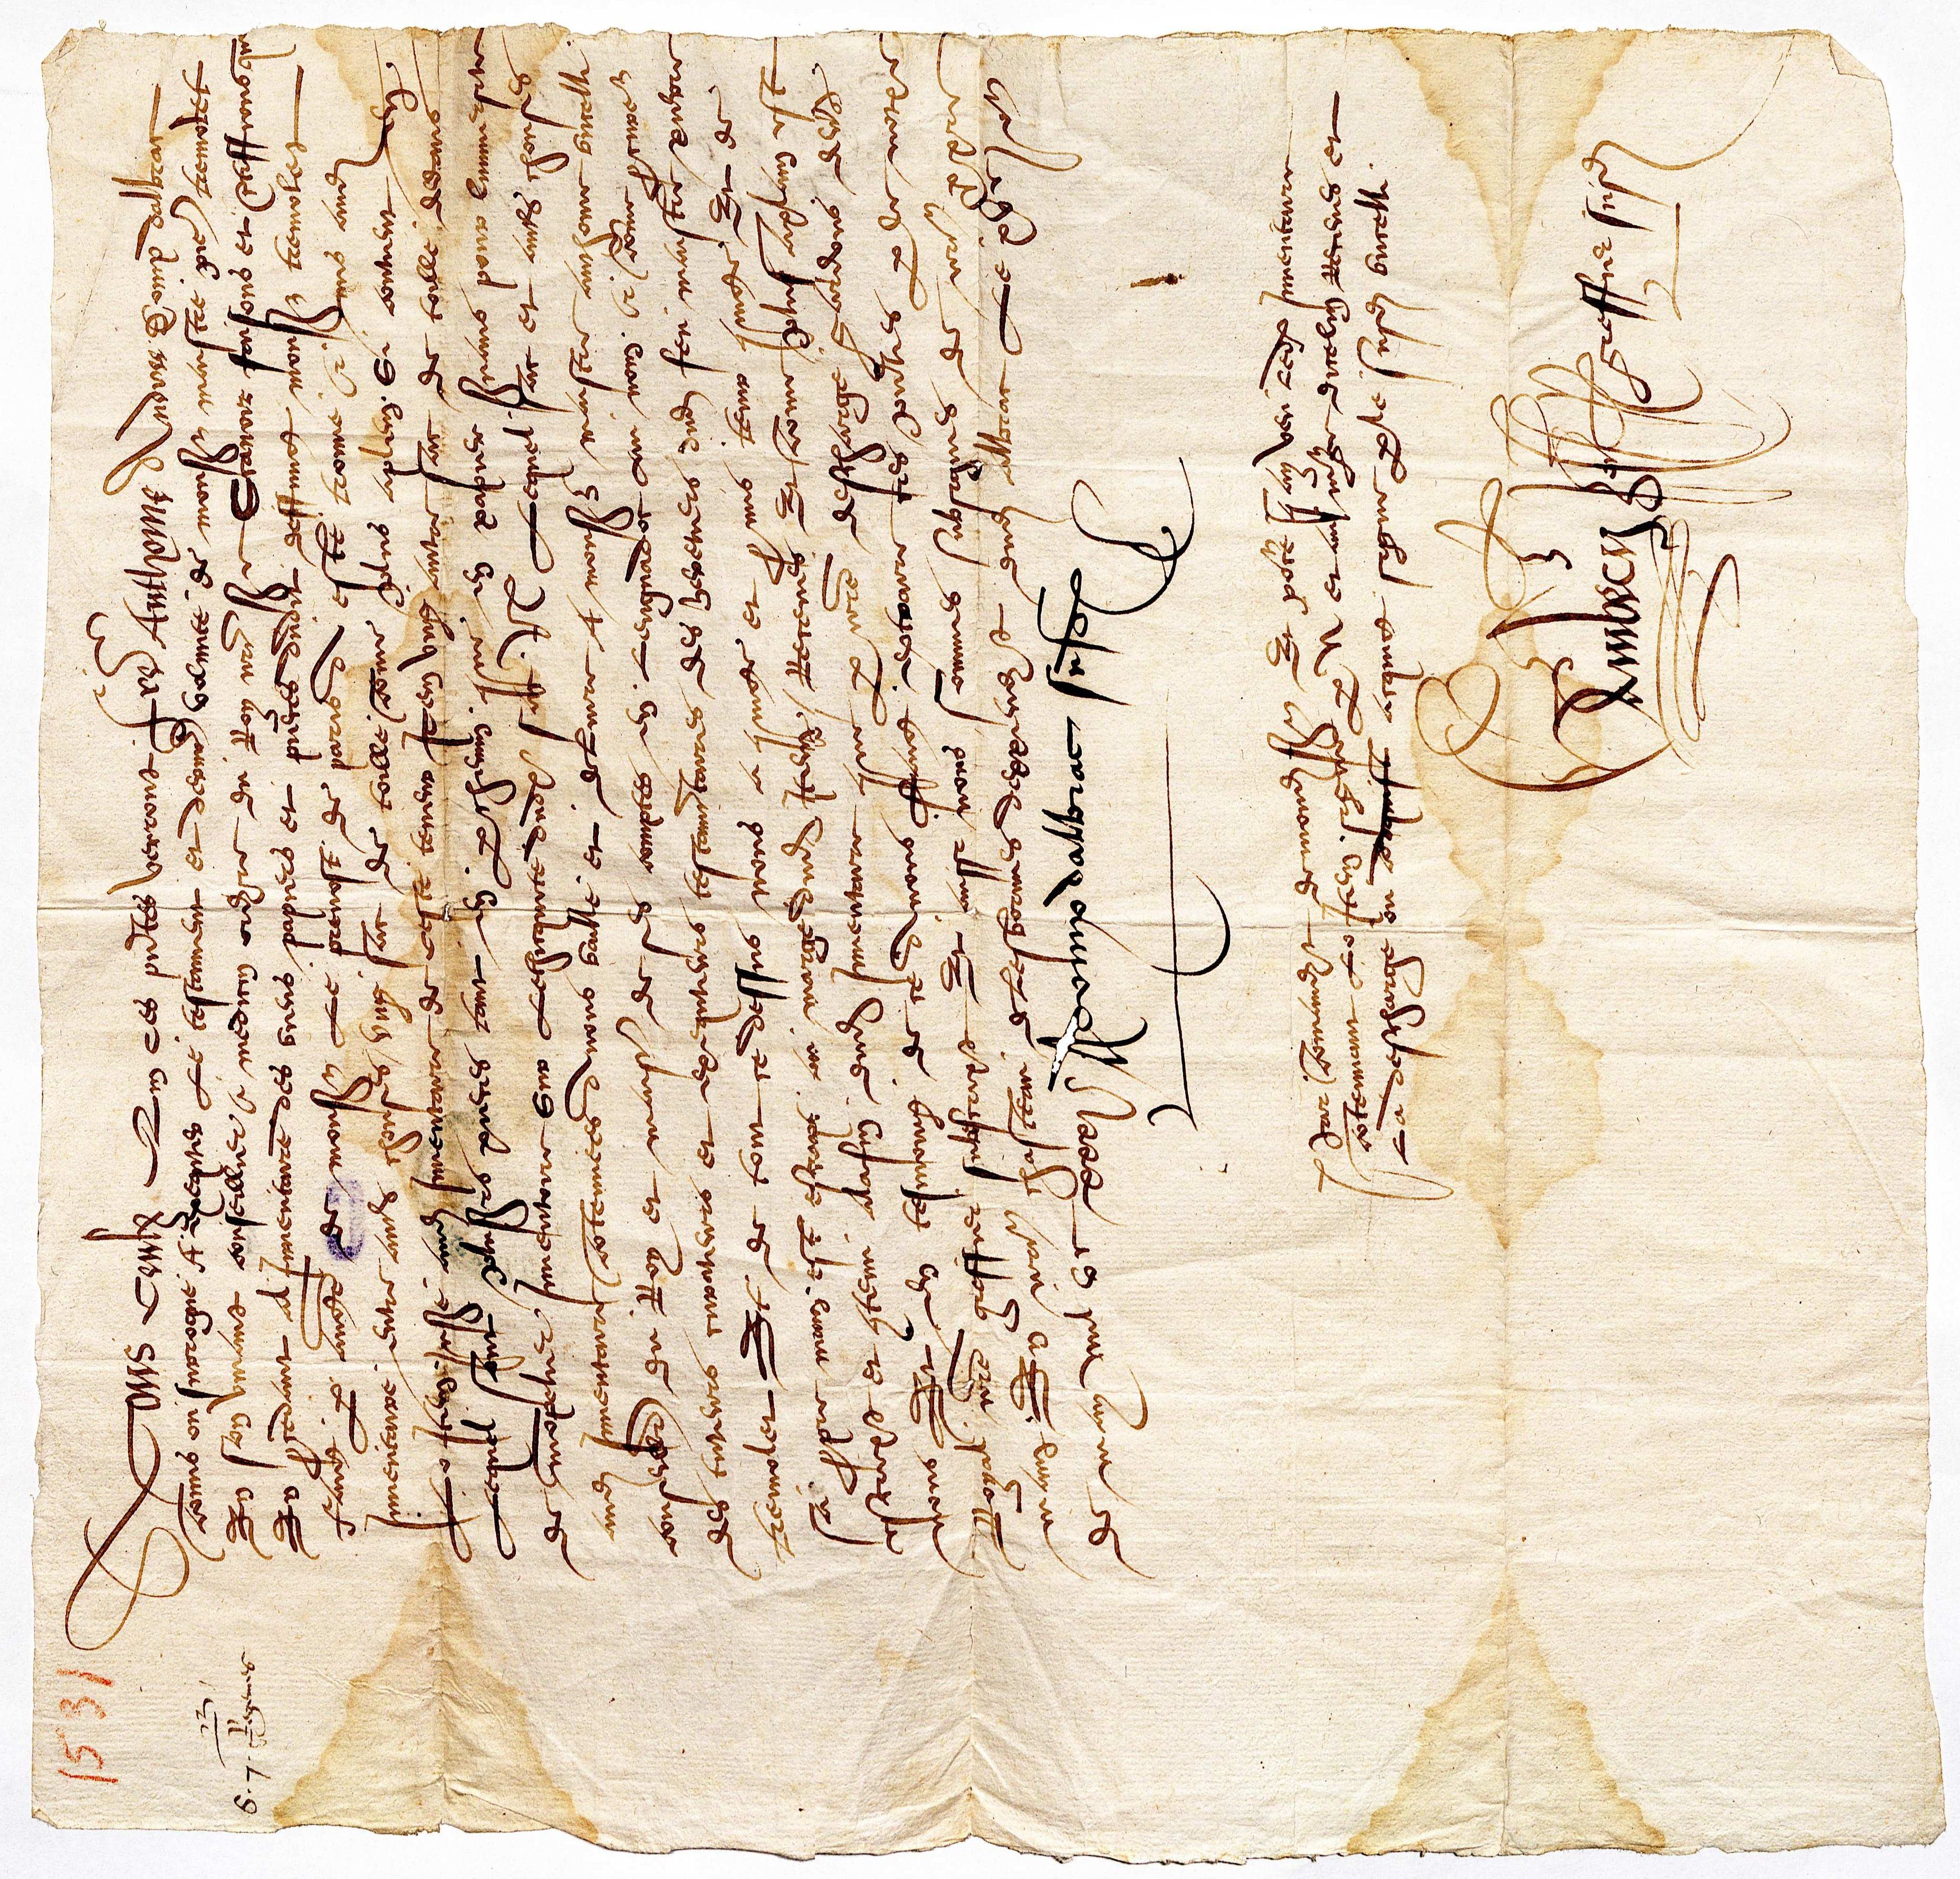
\includegraphics[
	angle=270,
	origin=c,
	width=\textwidth,
	height=0.82\textheight,
	keepaspectratio
	]{images/C4_01.jpg}
	\caption[Restitution à l'Université des papiers de Pierre Trémolet]
	{\enquote{Restitution de papiers appartenant à l'Université et trouvés dans la succession de feu Pierre Trémolet, docteur décédé à Paris}, 15 mai 1531, recto, Montpellier, Archives historiques de la Faculté de médecine, C~4 (ancienne cote : sac~7~B). Numérisation : Clara Martin.}
	\label{fig:c4-recto}
\end{figure}

\begin{figure}[p]
	\centering
	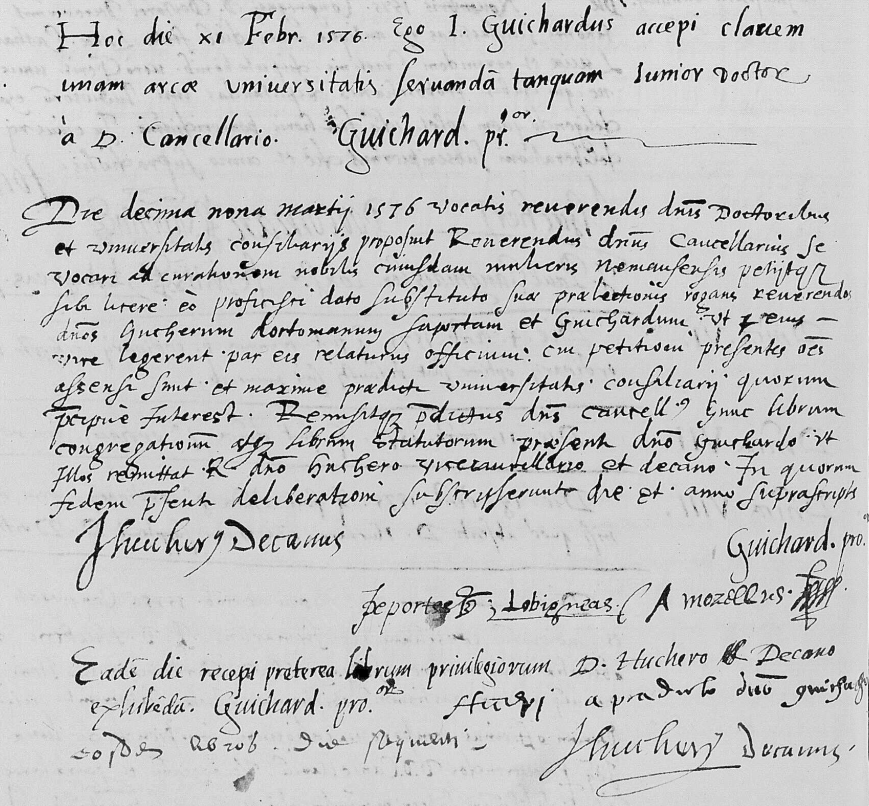
\includegraphics[
	width=\textwidth,
	height=0.78\textheight,
	keepaspectratio
	]{images/S8_f90v.png}
	\caption[Remise d'une clé du coffre et du livre des privilèges au procureur Guichard]
	{\enquote{Reconnaissance par le procureur Guichard de la remise d'une clé du coffre et du livre des privilèges}, 11 février 1576, détail du fol.~90~v\textsuperscript{o} recadré sur le passage concerné, dans le \emph{Liber congregationum Universitatis Monspeliensis}, registre des délibérations, actes et examens, 1557--1598, Montpellier, Archives historiques de la Faculté de médecine, S~8. Numérisation : Clara Martin.}
	\label{fig:s8-f90v}
\end{figure}

\begin{figure}[p]
	\centering
	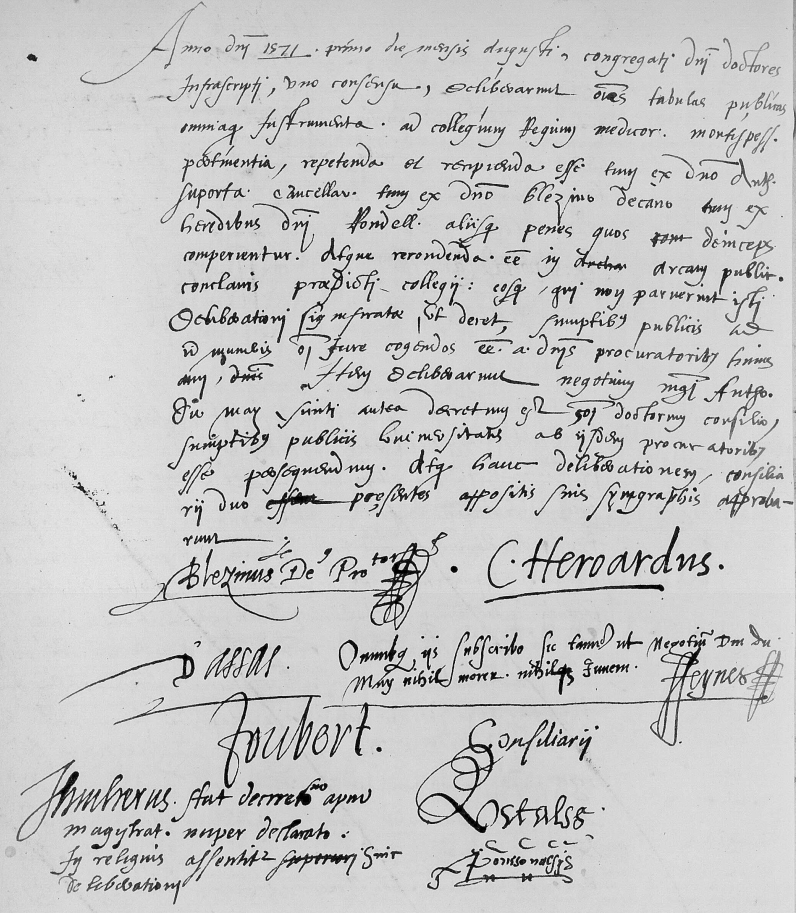
\includegraphics[
	width=\textwidth,
	height=0.78\textheight,
	keepaspectratio
	]{images/S8_f51.png}
	\caption[Réunion des archives dans le coffre public de la salle du Collège]
	{\enquote{Délibération prescrivant la récupération des actes et registres appartenant au Collège des médecins et leur dépôt dans le coffre public de la salle du Collège}, 1\textsuperscript{er} août 1571, fol.~51~v\textsuperscript{o}, dans le \emph{Liber congregationum Universitatis Monspeliensis}, registre des délibérations, actes et examens, 1557--1598, Montpellier, Archives historiques de la Faculté de médecine, S~8. Numérisation : Clara Martin.}
	\label{fig:s8-f51v}
\end{figure}

\begin{figure}[p]
	\centering
	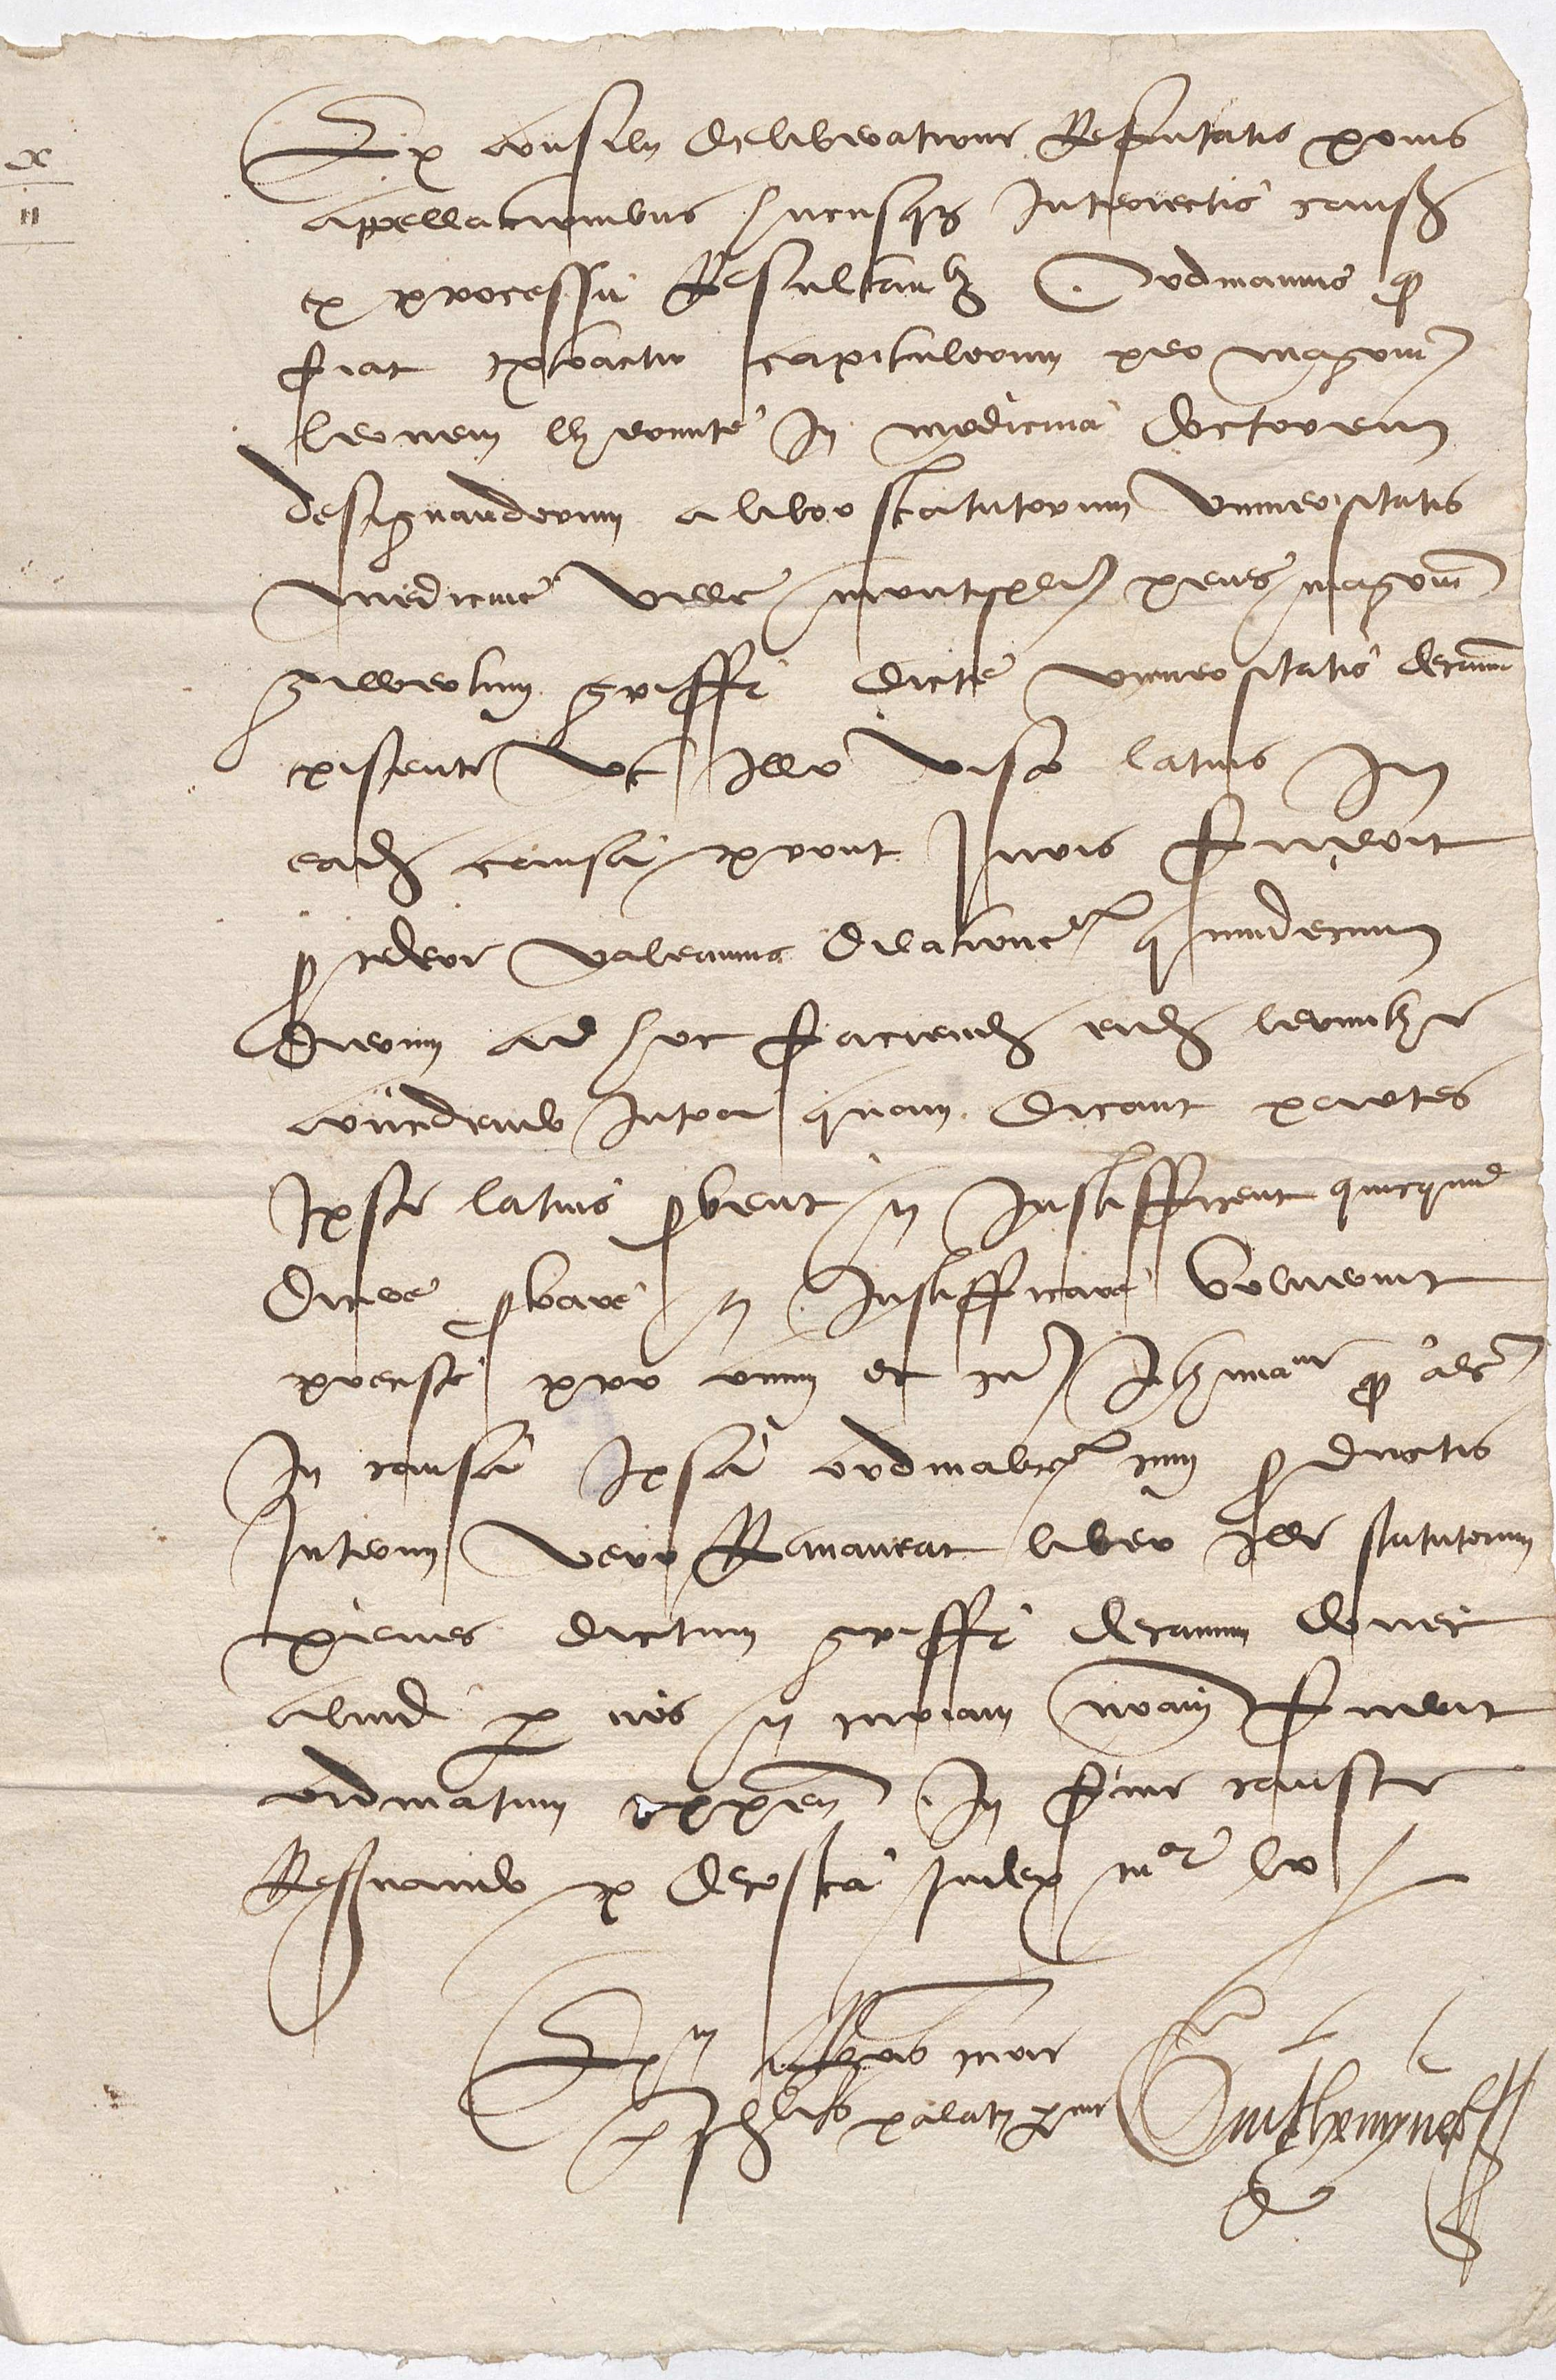
\includegraphics[
	width=\textwidth,
	height=0.78\textheight,
	keepaspectratio
	]{images/C9.jpg}
	\caption[Autorisation donnée à Lermite de faire des extraits des statuts]
	{\enquote{Procès-verbal d'une délibération en vertu de laquelle Lermite, docteur, est autorisé à faire certains extraits des statuts, dans les registres qui sont entre les mains du doyen Gilbert Griffi}, s. d., Montpellier, Archives historiques de la Faculté de médecine, C~9 (ancienne cote : sac~11~X). Numérisation : Clara Martin.}
	\label{fig:c9}
\end{figure}

\begin{figure}[p]
	\centering
	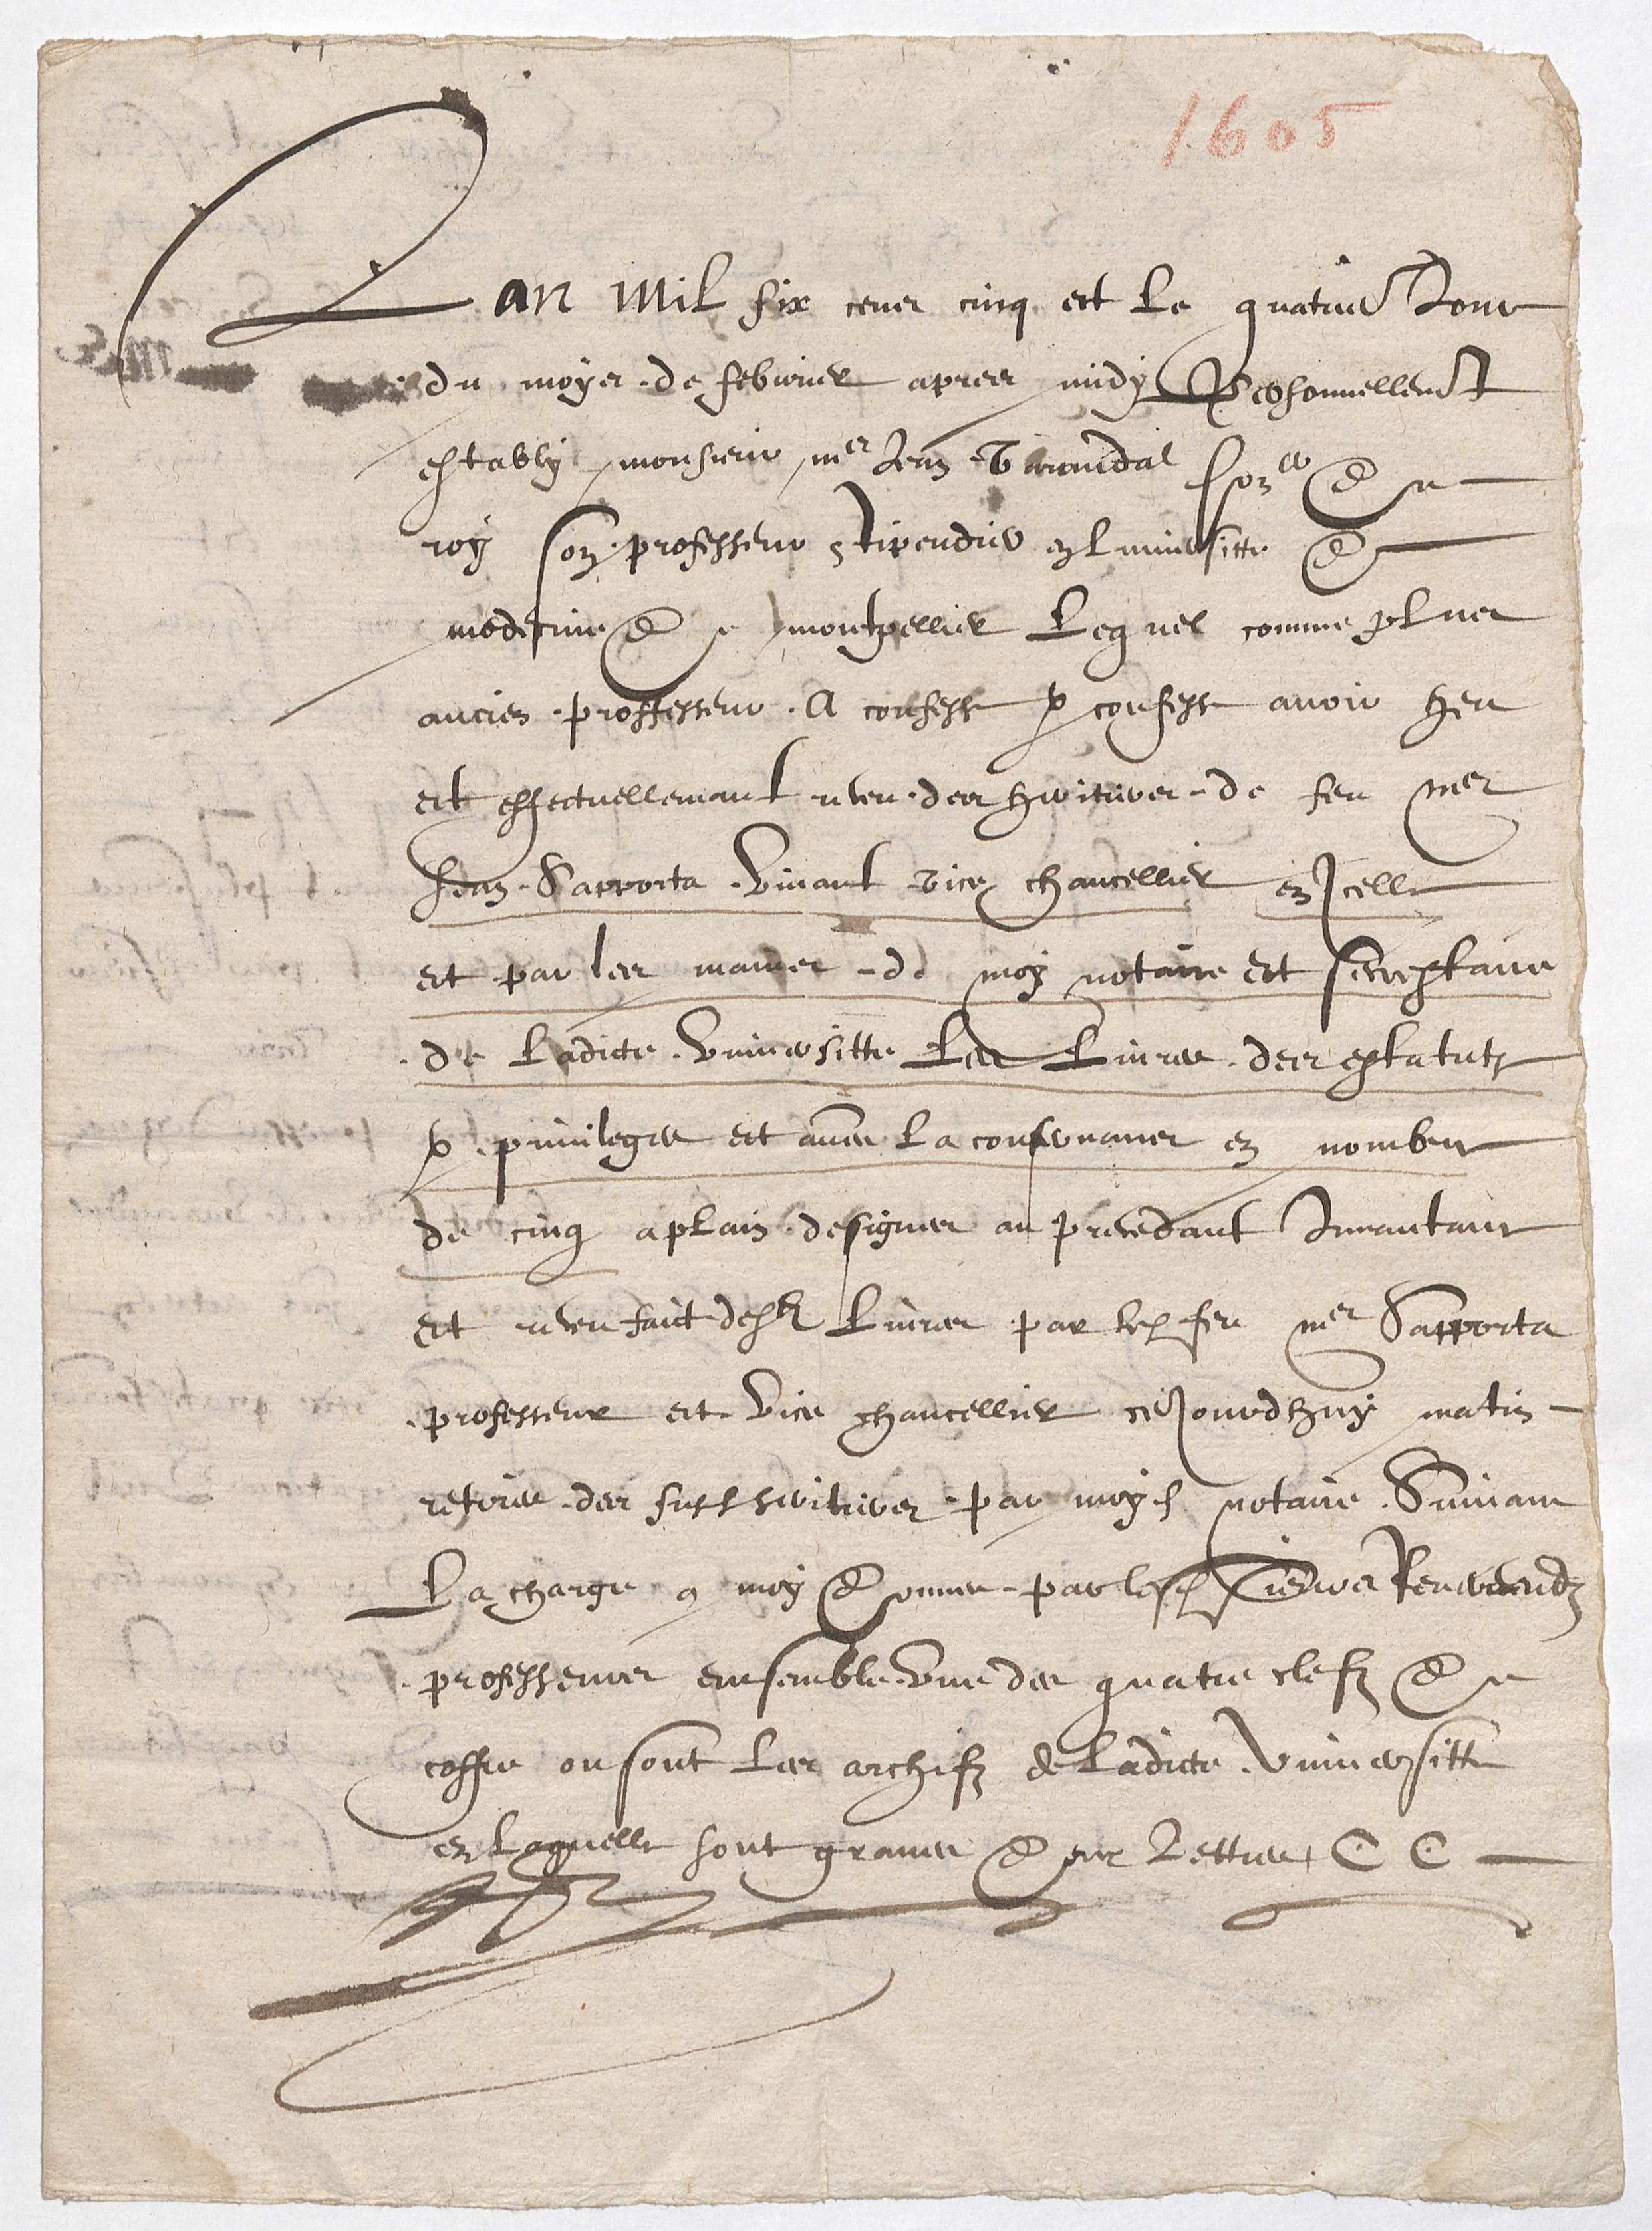
\includegraphics[
	width=\textwidth,
	height=0.78\textheight,
	keepaspectratio
	]{images/C35_01.jpg}
	\caption[Remise des archives à Jean Varanda en qualité de plus ancien docteur]
	{\enquote{Remise des archives à Jean Varanda en qualité de plus ancien docteur}, 4 février 1605, première vue, Montpellier, Archives historiques de la Faculté de médecine, C~35. Numérisation : Clara Martin.}
	\label{fig:c35-01}
\end{figure}

\clearpage

\begin{landscape}
	\begin{figure}[p]
		\centering
		
		\rotatebox{180}{%
			\begin{minipage}{\linewidth}
				\centering
				
				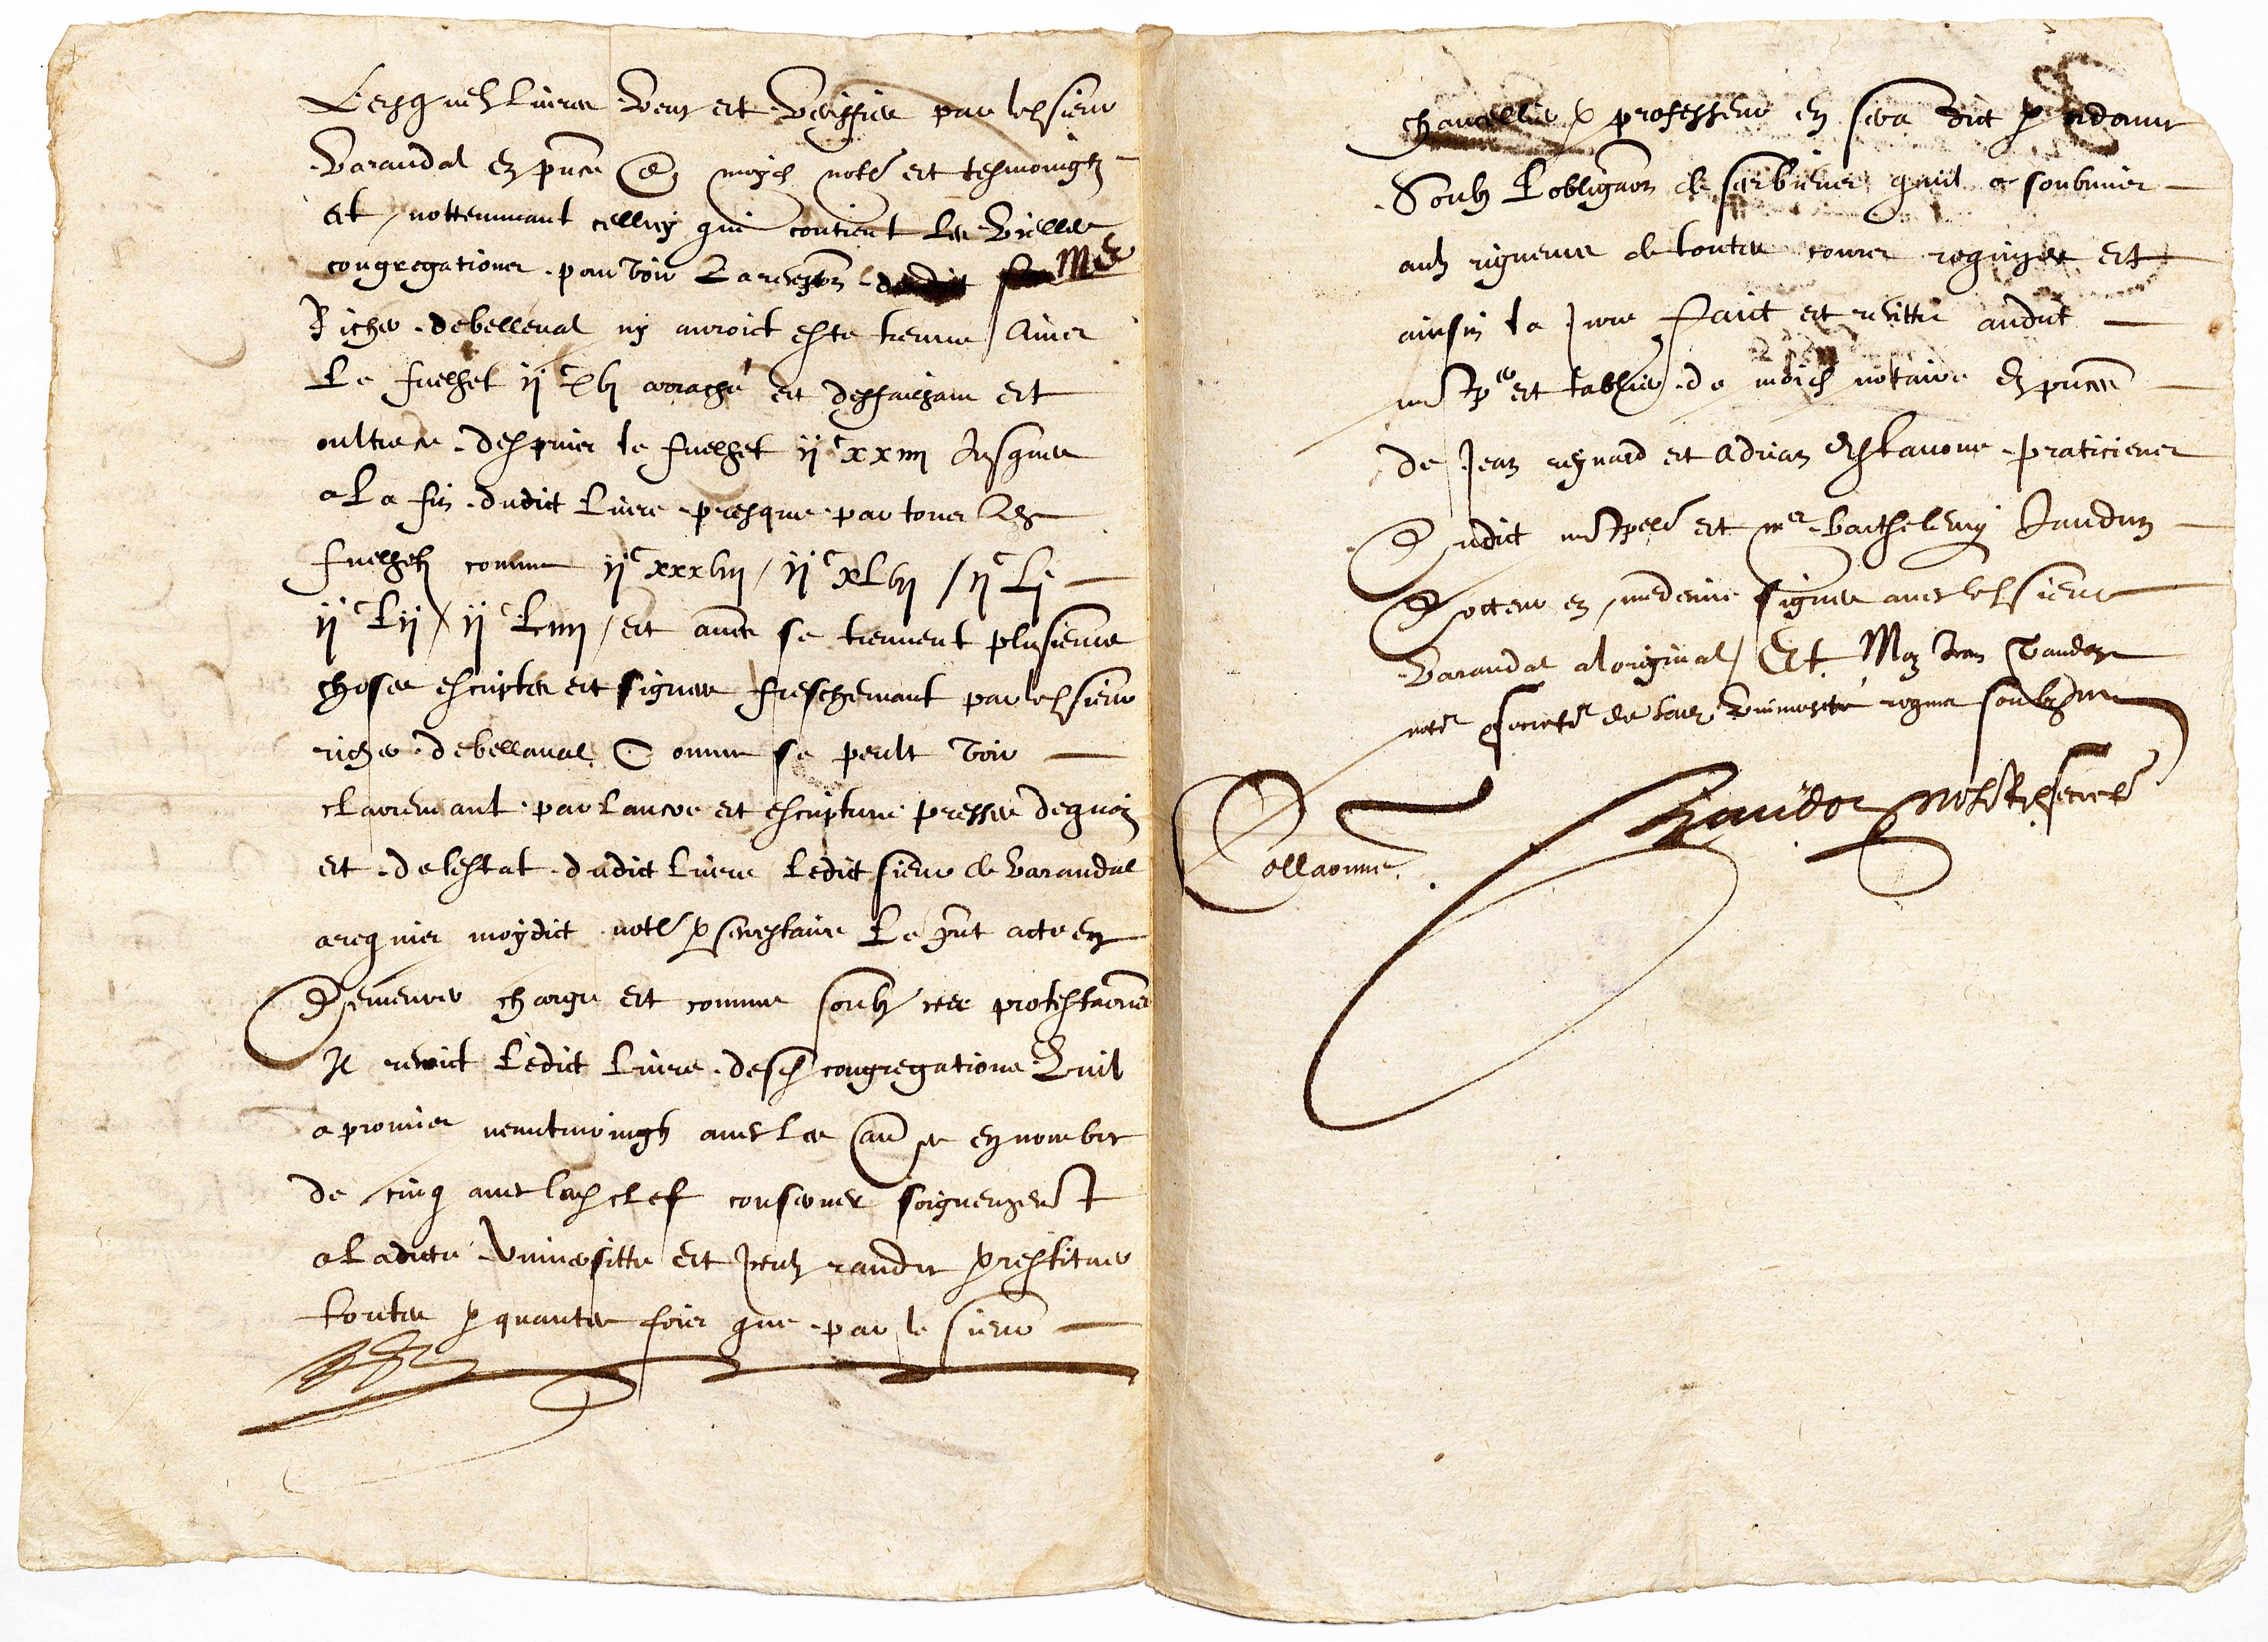
\includegraphics[
				width=0.92\linewidth,
				keepaspectratio
				]{images/C35_02.jpg}
				
				\captionof{figure}
				[Remise des archives à Jean Varanda en qualité de plus ancien docteur]
				{\enquote{Remise des archives à Jean Varanda en qualité de plus ancien docteur}, 4 février 1605, seconde vue, Montpellier, Archives historiques de la Faculté de médecine, C~35. Numérisation : Clara Martin.}
				
				\label{fig:c35-02}
				
			\end{minipage}%
		}
		
	\end{figure}
\end{landscape}

\begin{figure}[p]
	\centering
	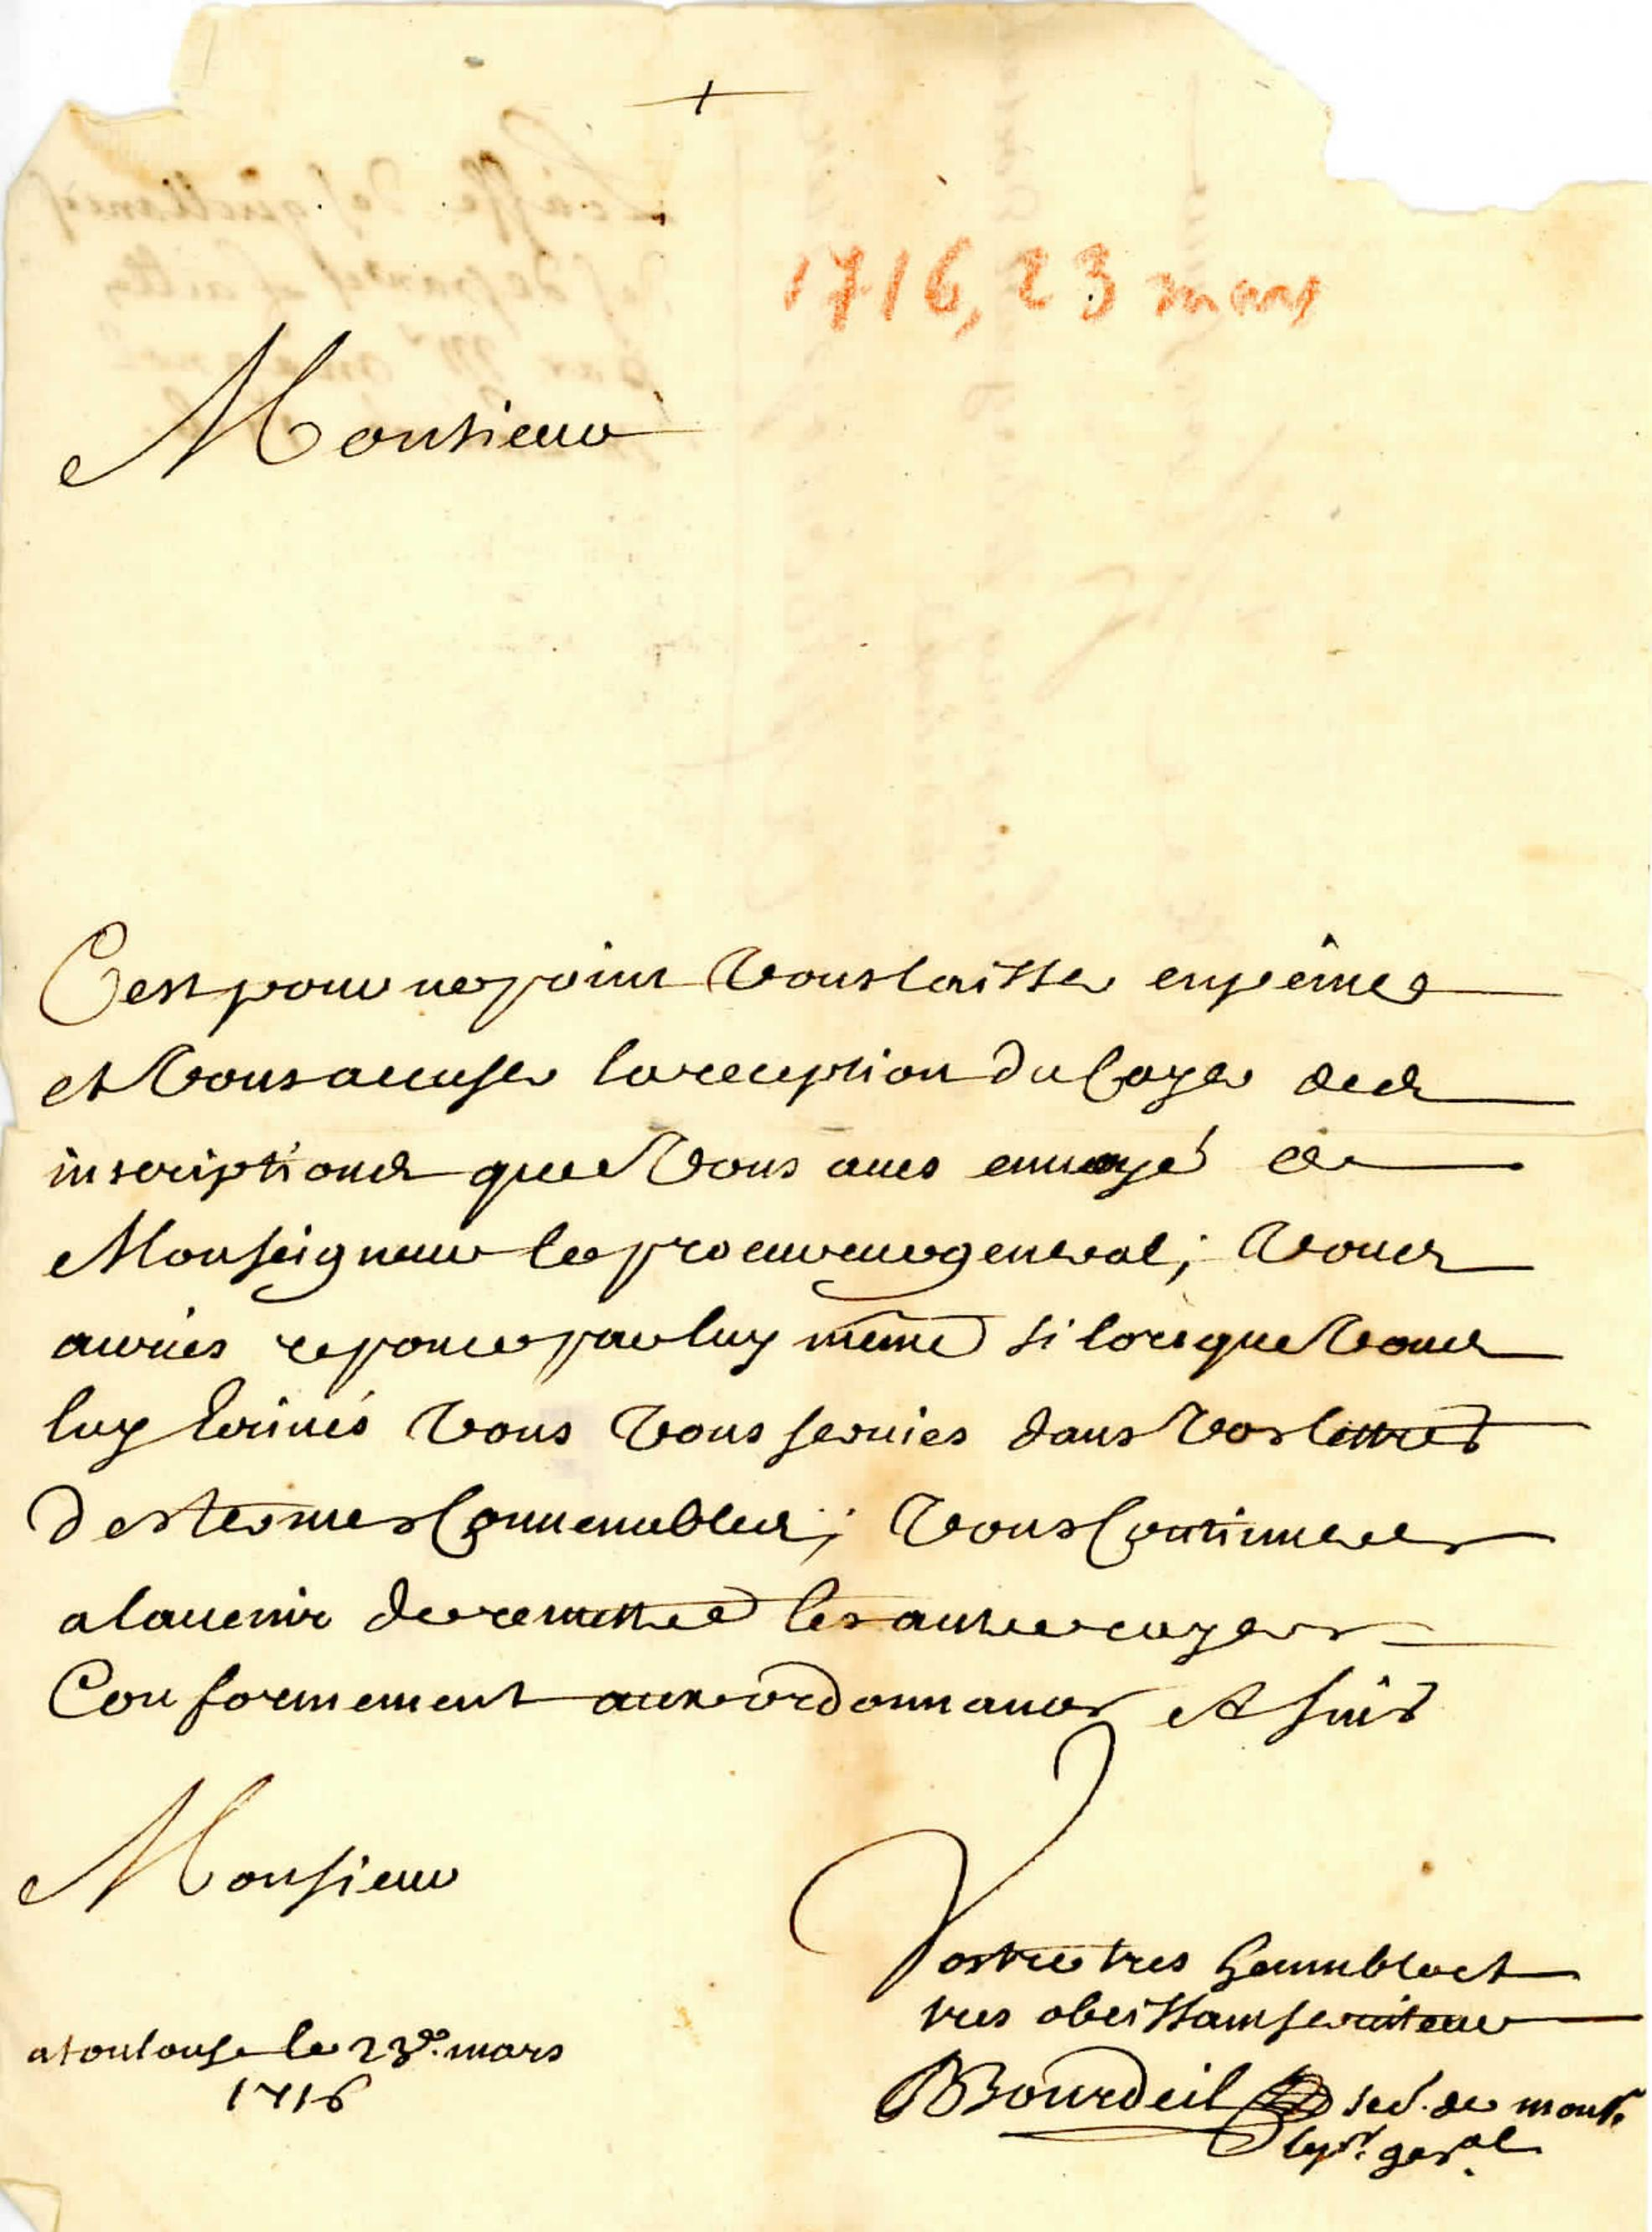
\includegraphics[
	width=\textwidth,
	height=0.78\textheight,
	keepaspectratio
	]{images/F24_01.jpg}
	\caption[Lettre accusant réception d'un registre d'inscription, recto]
	{\enquote{Lettre du sieur de Bourdeil, secrétaire de M. le Procureur général, pour accuser réception d'un registre d'inscription}, recto, Toulouse, 23 mars 1716, Montpellier, Archives historiques de la Faculté de médecine, F~24. Numérisation : Clara Martin.}
	\label{fig:f24-01}
\end{figure}

\begin{figure}[p]
	\centering
	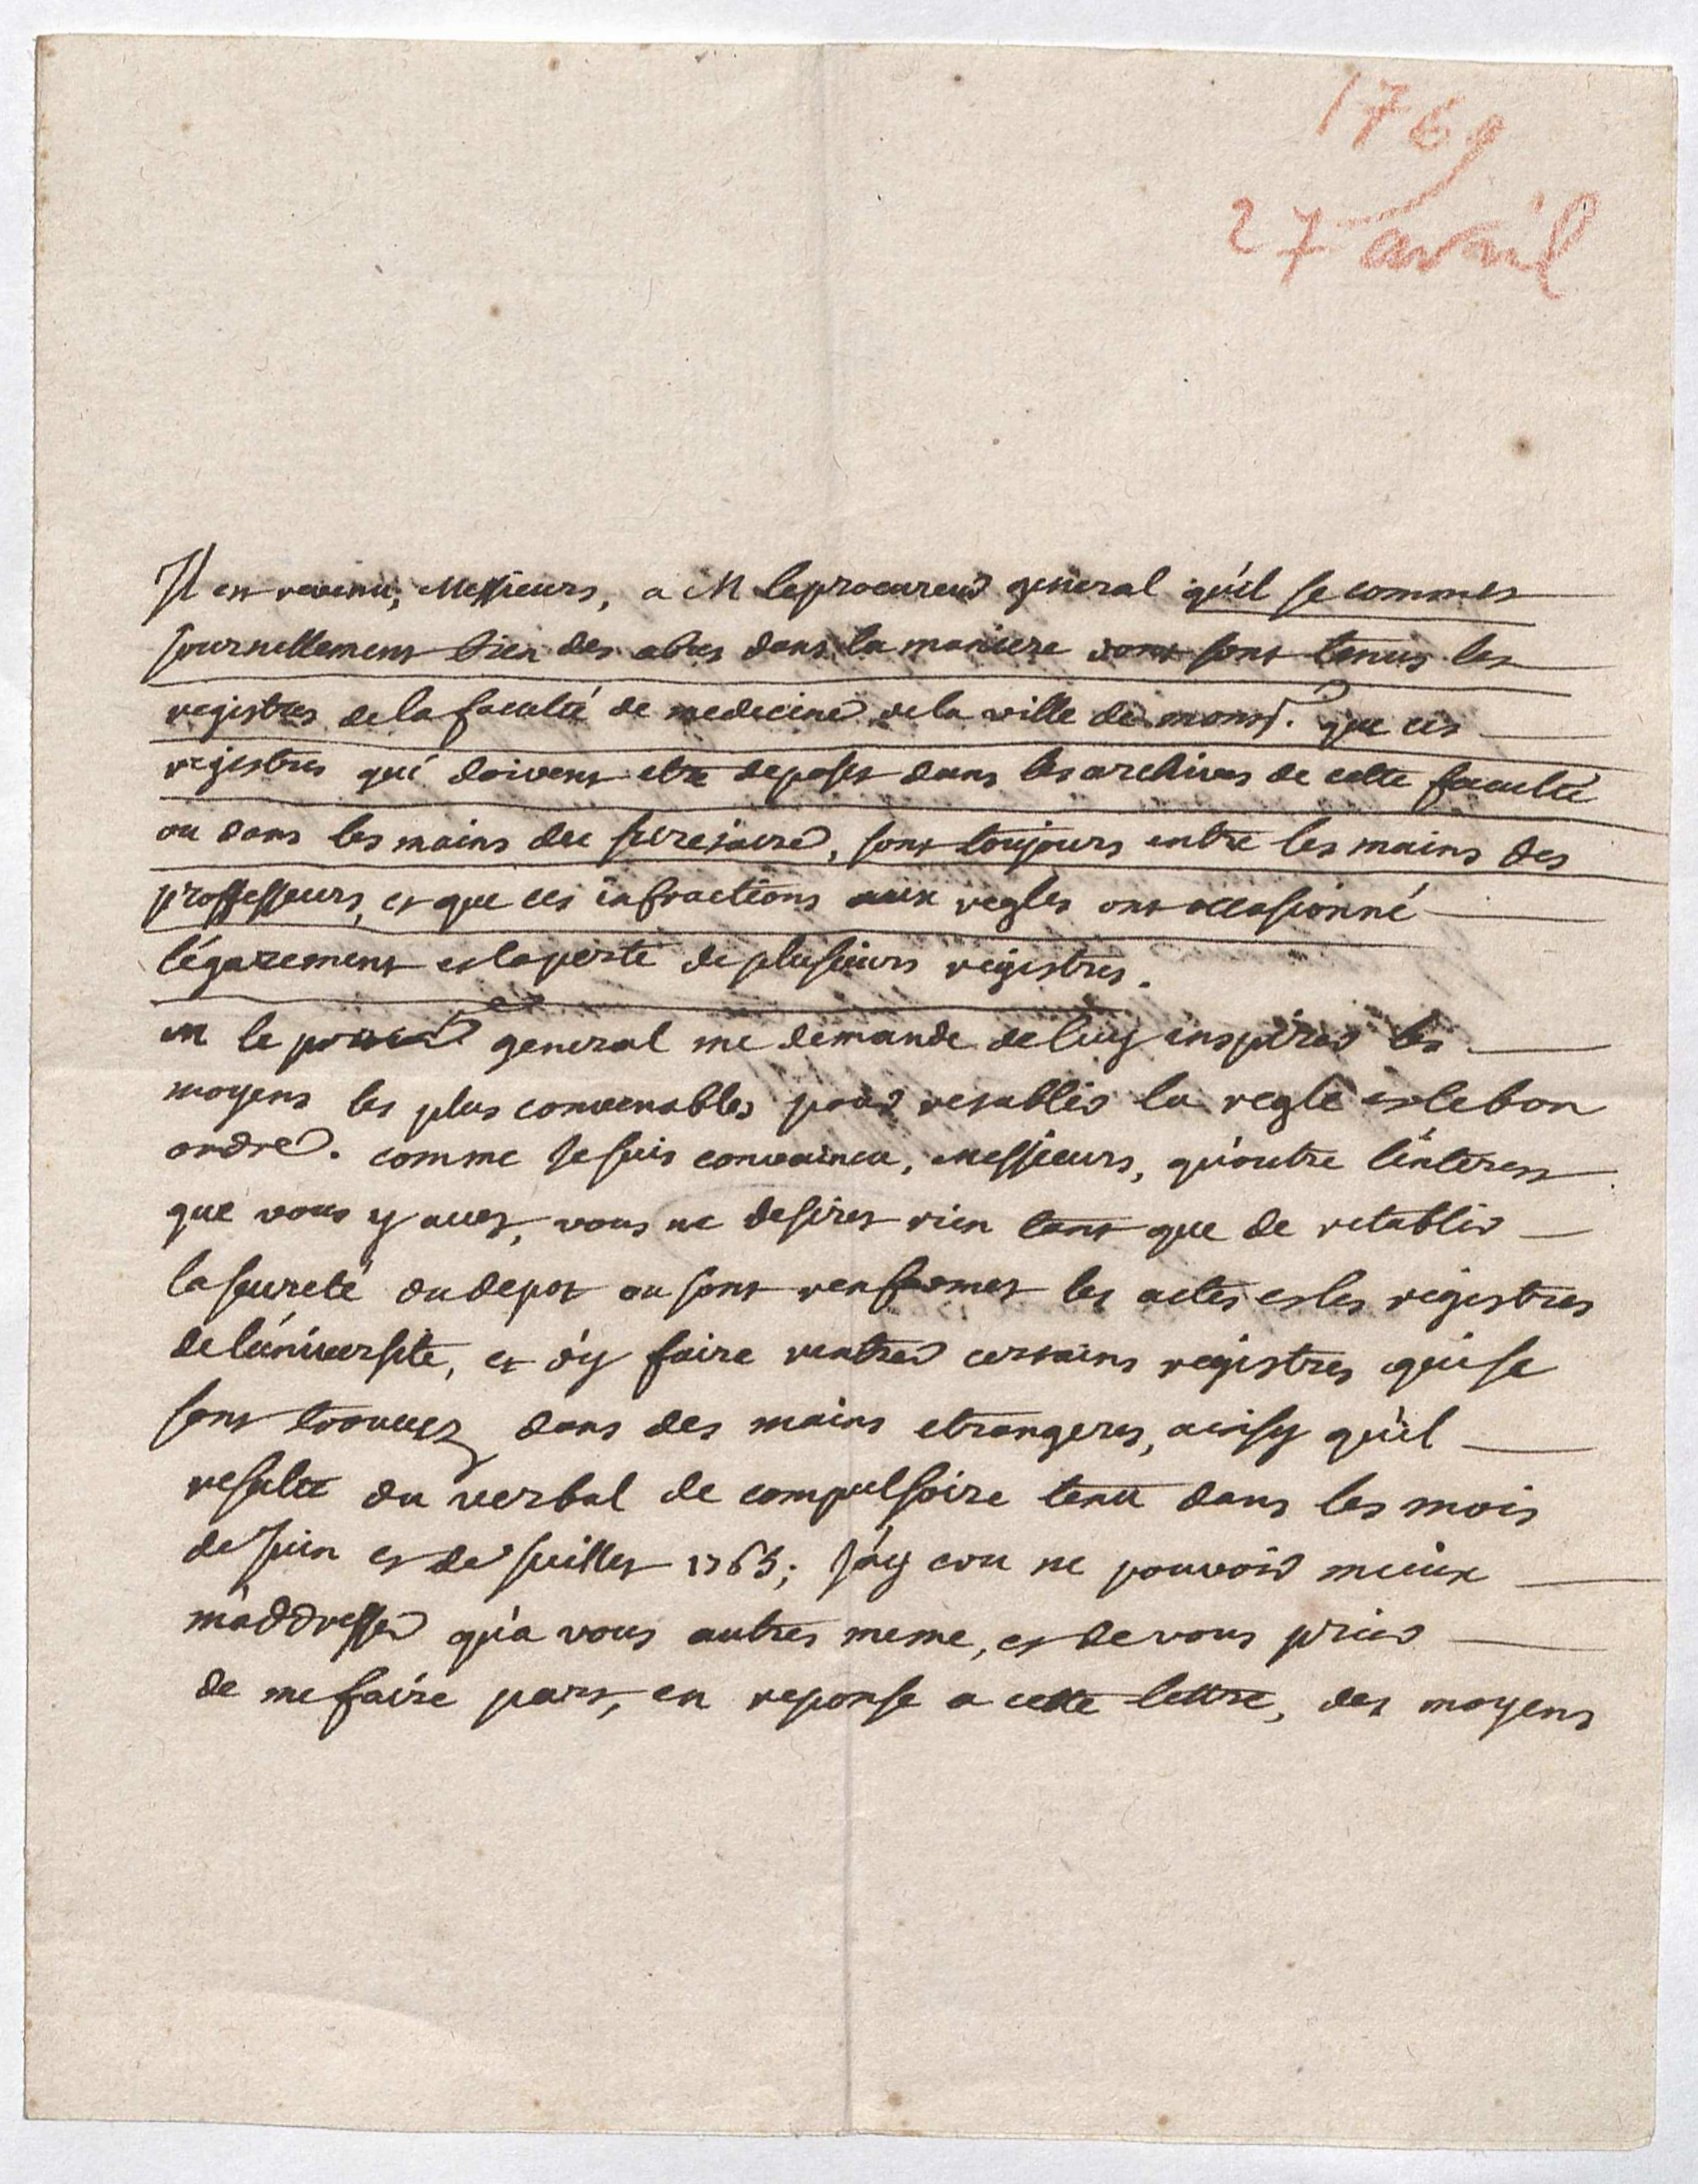
\includegraphics[
	width=\textwidth,
	height=0.78\textheight,
	keepaspectratio
	]{images/F54_19.jpg}
	\caption[Lettre relative à la mauvaise tenue des archives, première vue]
	{\enquote{Lettre écrite au nom du procureur général au sujet de la mauvaise tenue des archives de la Faculté et sur les mesures qu'il serait indispensable de prendre pour éviter la perte des documents}, première vue, 27 avril 1769, sans lieu, Montpellier, Archives historiques de la Faculté de médecine, F~54. Numérisation : Clara Martin.}
	\label{fig:f54-19}
\end{figure}

\begin{figure}[p]
	\centering
	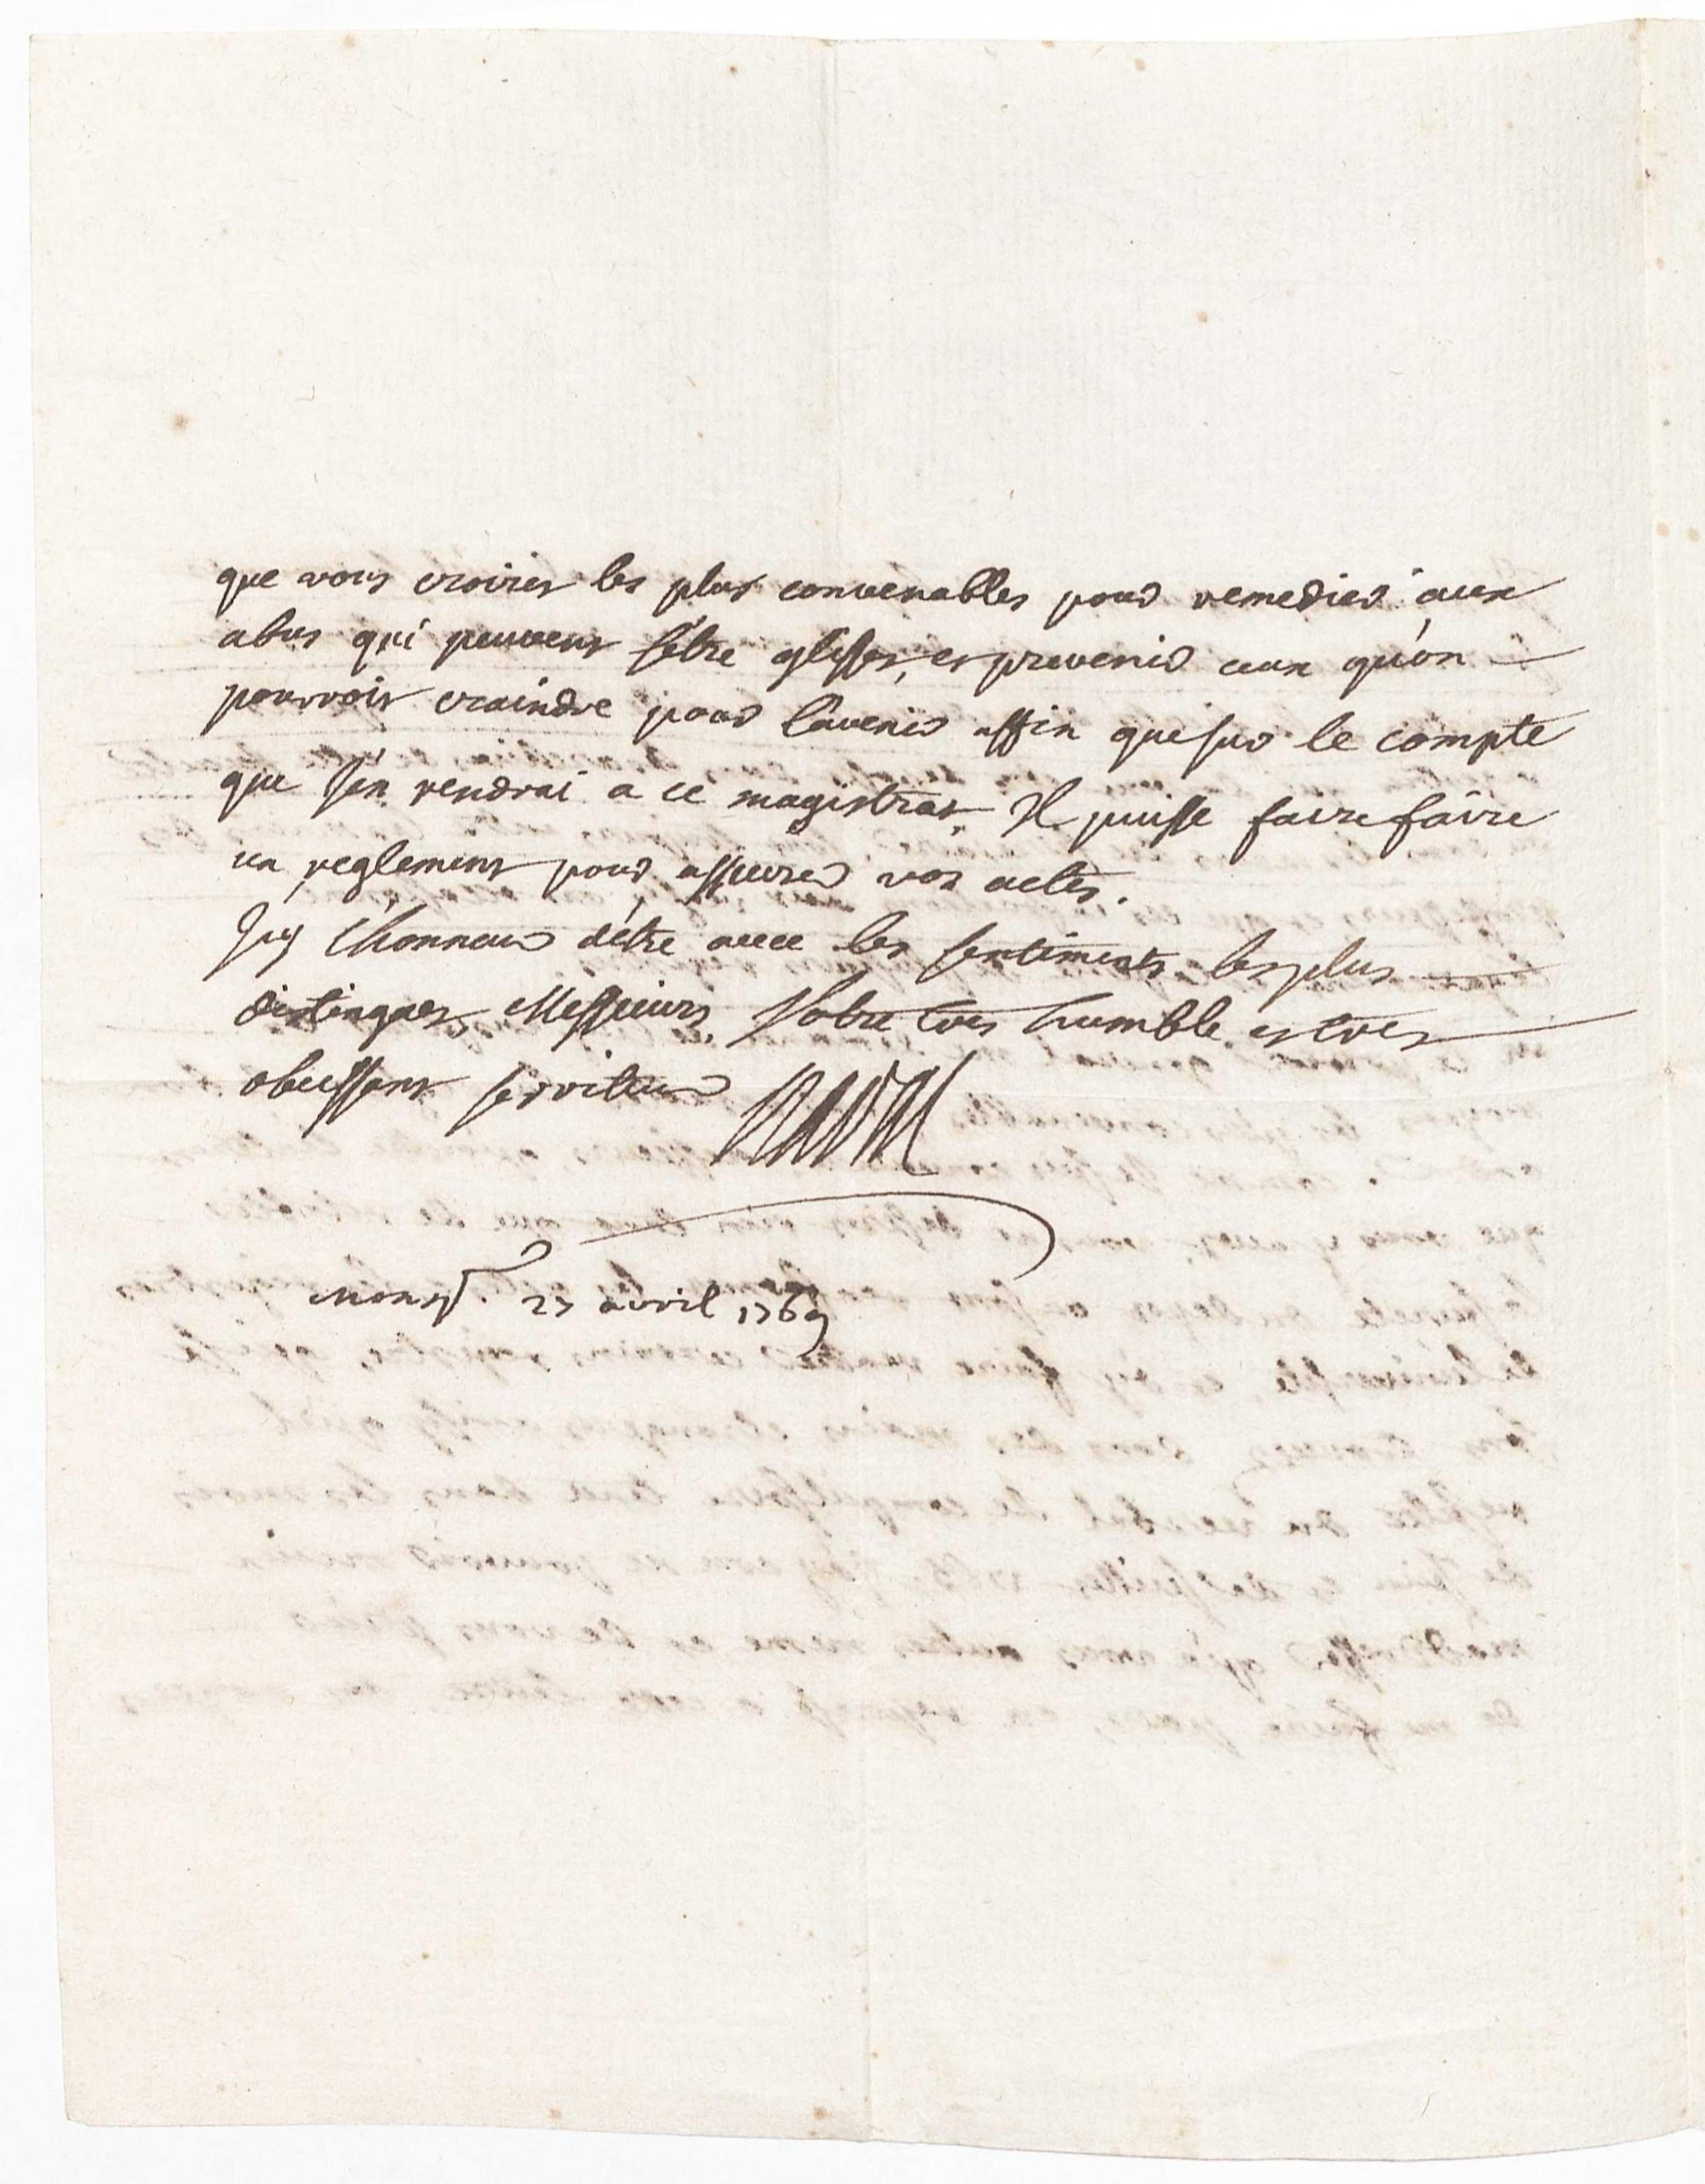
\includegraphics[
	width=\textwidth,
	height=0.78\textheight,
	keepaspectratio
	]{images/F54_20.jpg}
	\caption[Lettre relative à la mauvaise tenue des archives, seconde vue]
	{\enquote{Lettre écrite au nom du procureur général au sujet de la mauvaise tenue des archives de la Faculté et sur les mesures qu'il serait indispensable de prendre pour éviter la perte des documents}, seconde vue, 27 avril 1769, sans lieu, Montpellier, Archives historiques de la Faculté de médecine, F~54. Numérisation : Clara Martin.}
	\label{fig:f54-20}
\end{figure}

\begin{figure}[p]
	\centering
	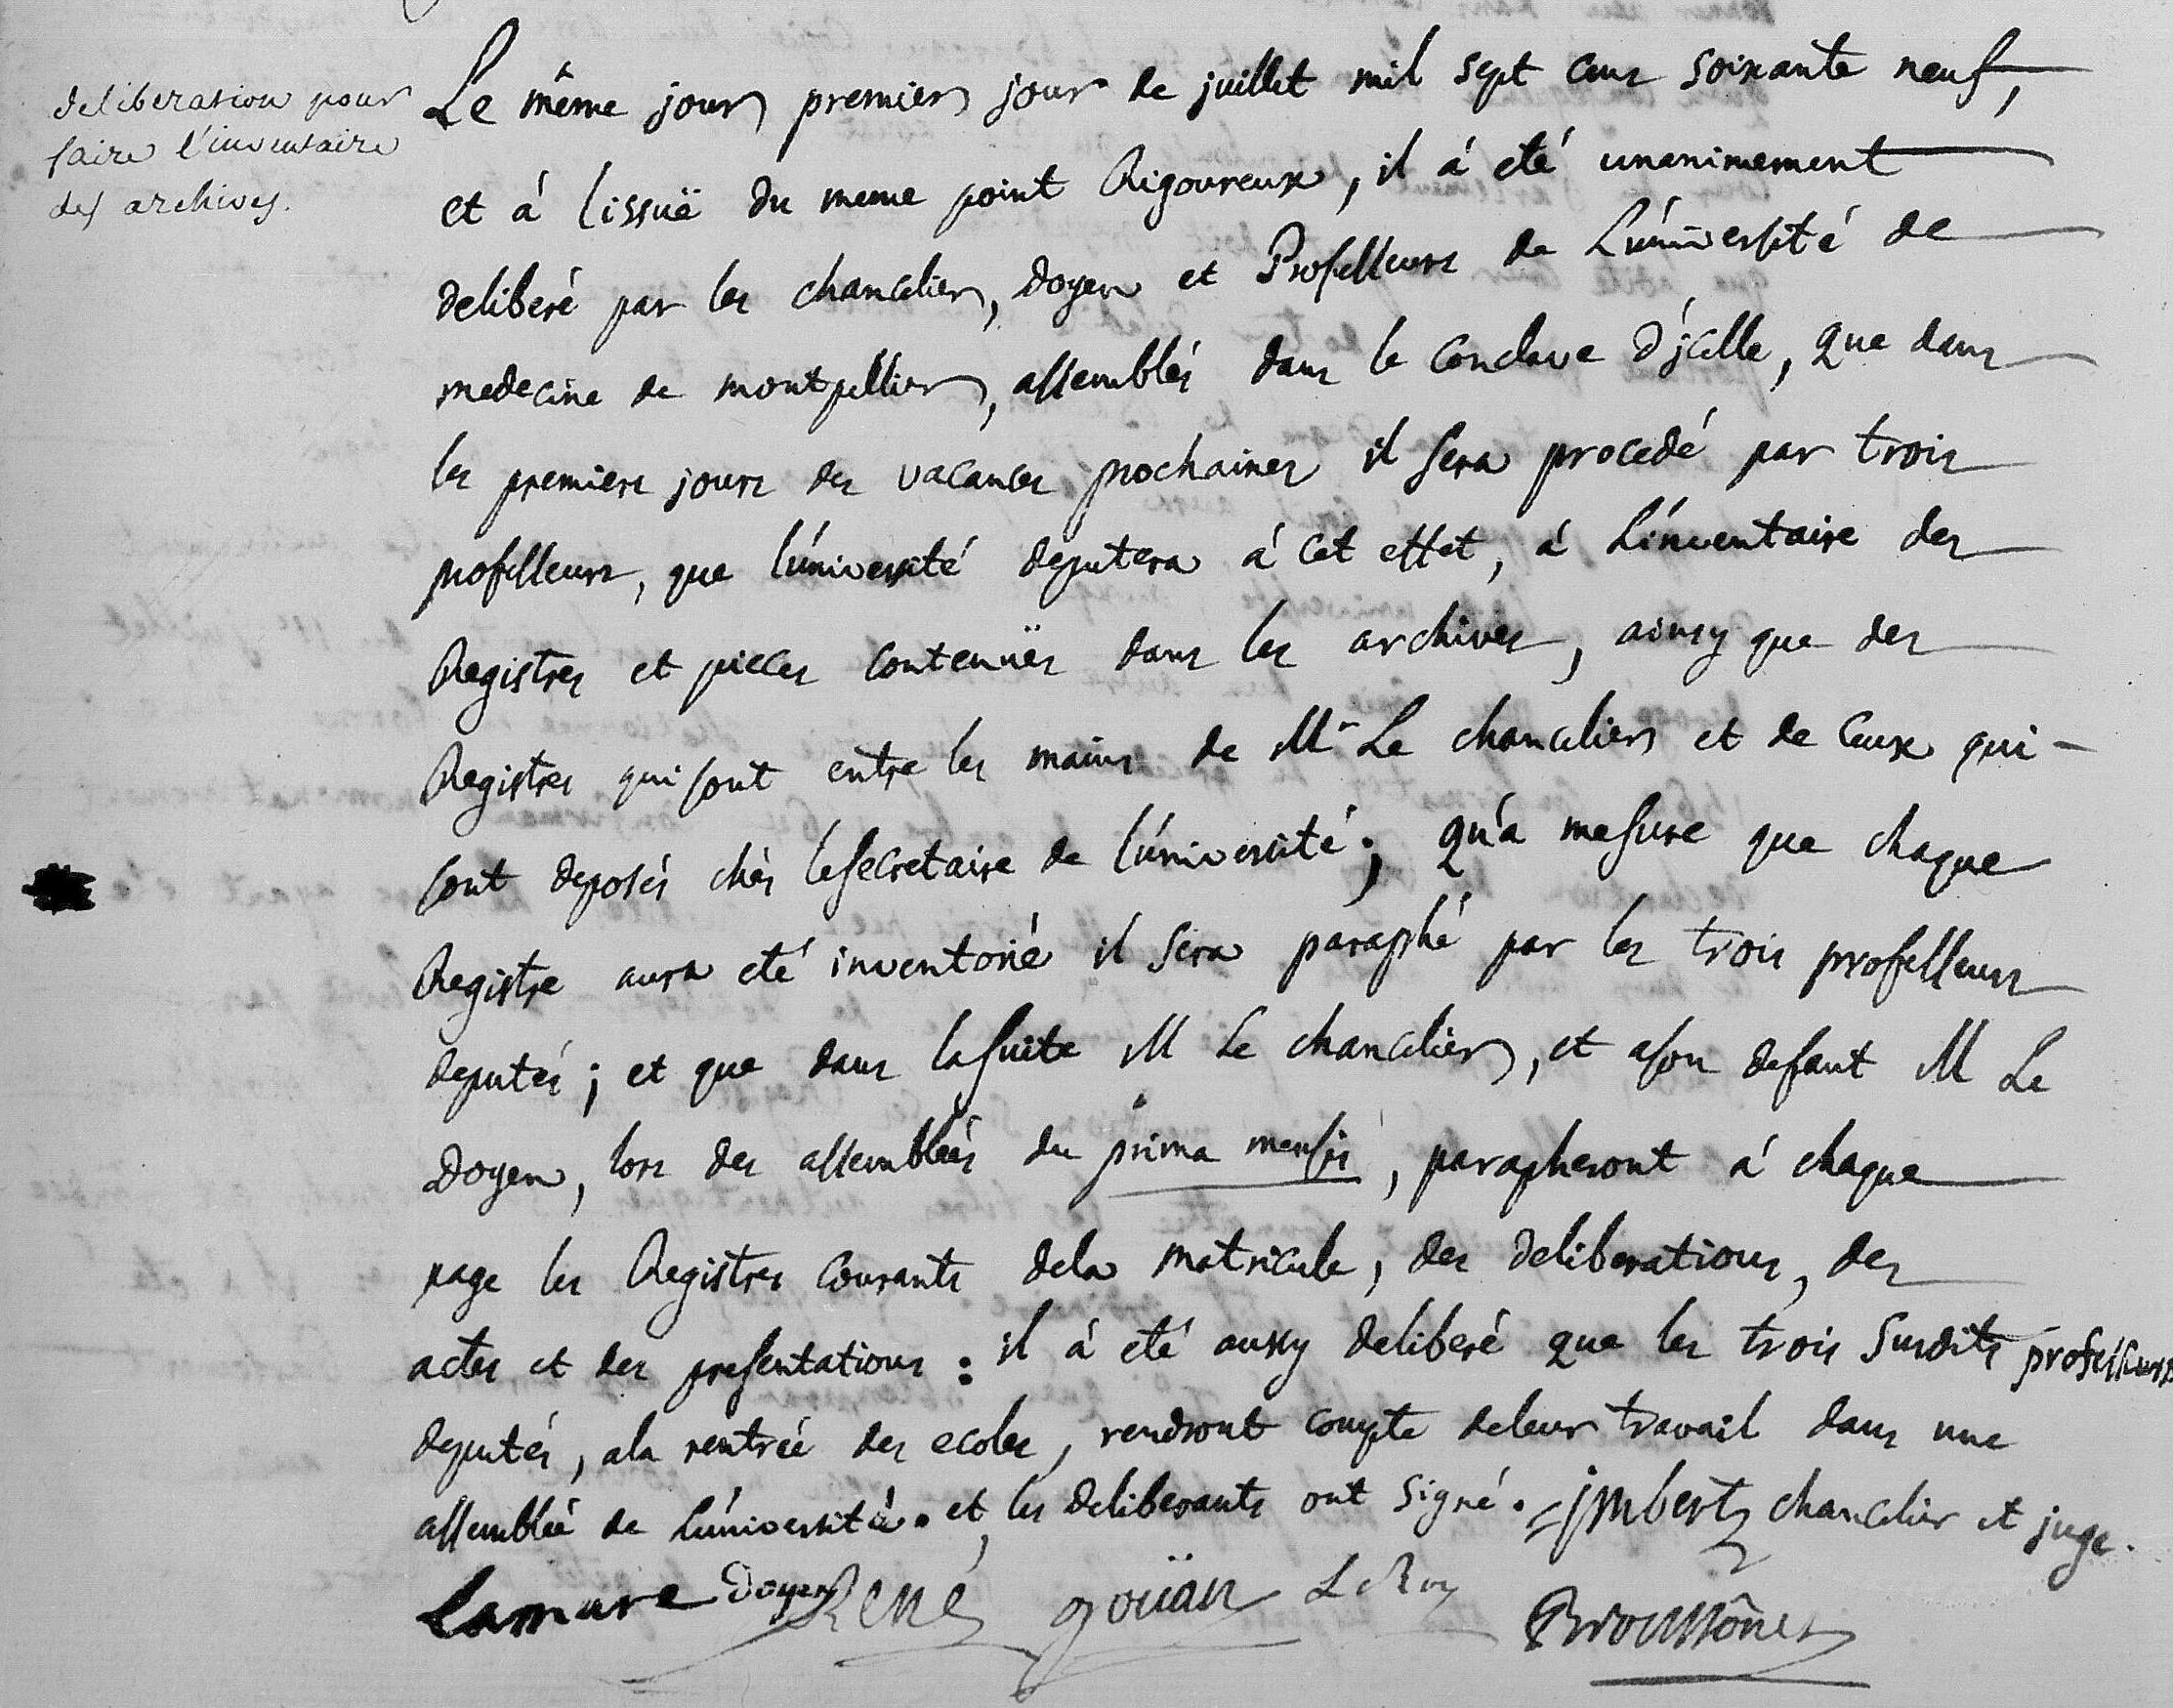
\includegraphics[
	width=\textwidth,
	height=0.78\textheight,
	keepaspectratio
	]{images/S17_p8.jpg}
	\caption[Délibération relative à la réalisation d'un nouvel inventaire, 1\textsuperscript{er} juillet 1769]
	{Délibération relative à la réalisation d'un nouvel inventaire des archives de la Faculté, 1\textsuperscript{er} juillet 1769, dans le \emph{Registre des délibérations. Suite du registre précédent} (15 octobre 1768--4 brumaire an III), Montpellier, Archives historiques de la Faculté de médecine, S~17. Numérisation : Clara Martin.}
	\label{fig:s17-p8}
\end{figure}

\begin{figure}[p]
	\centering
	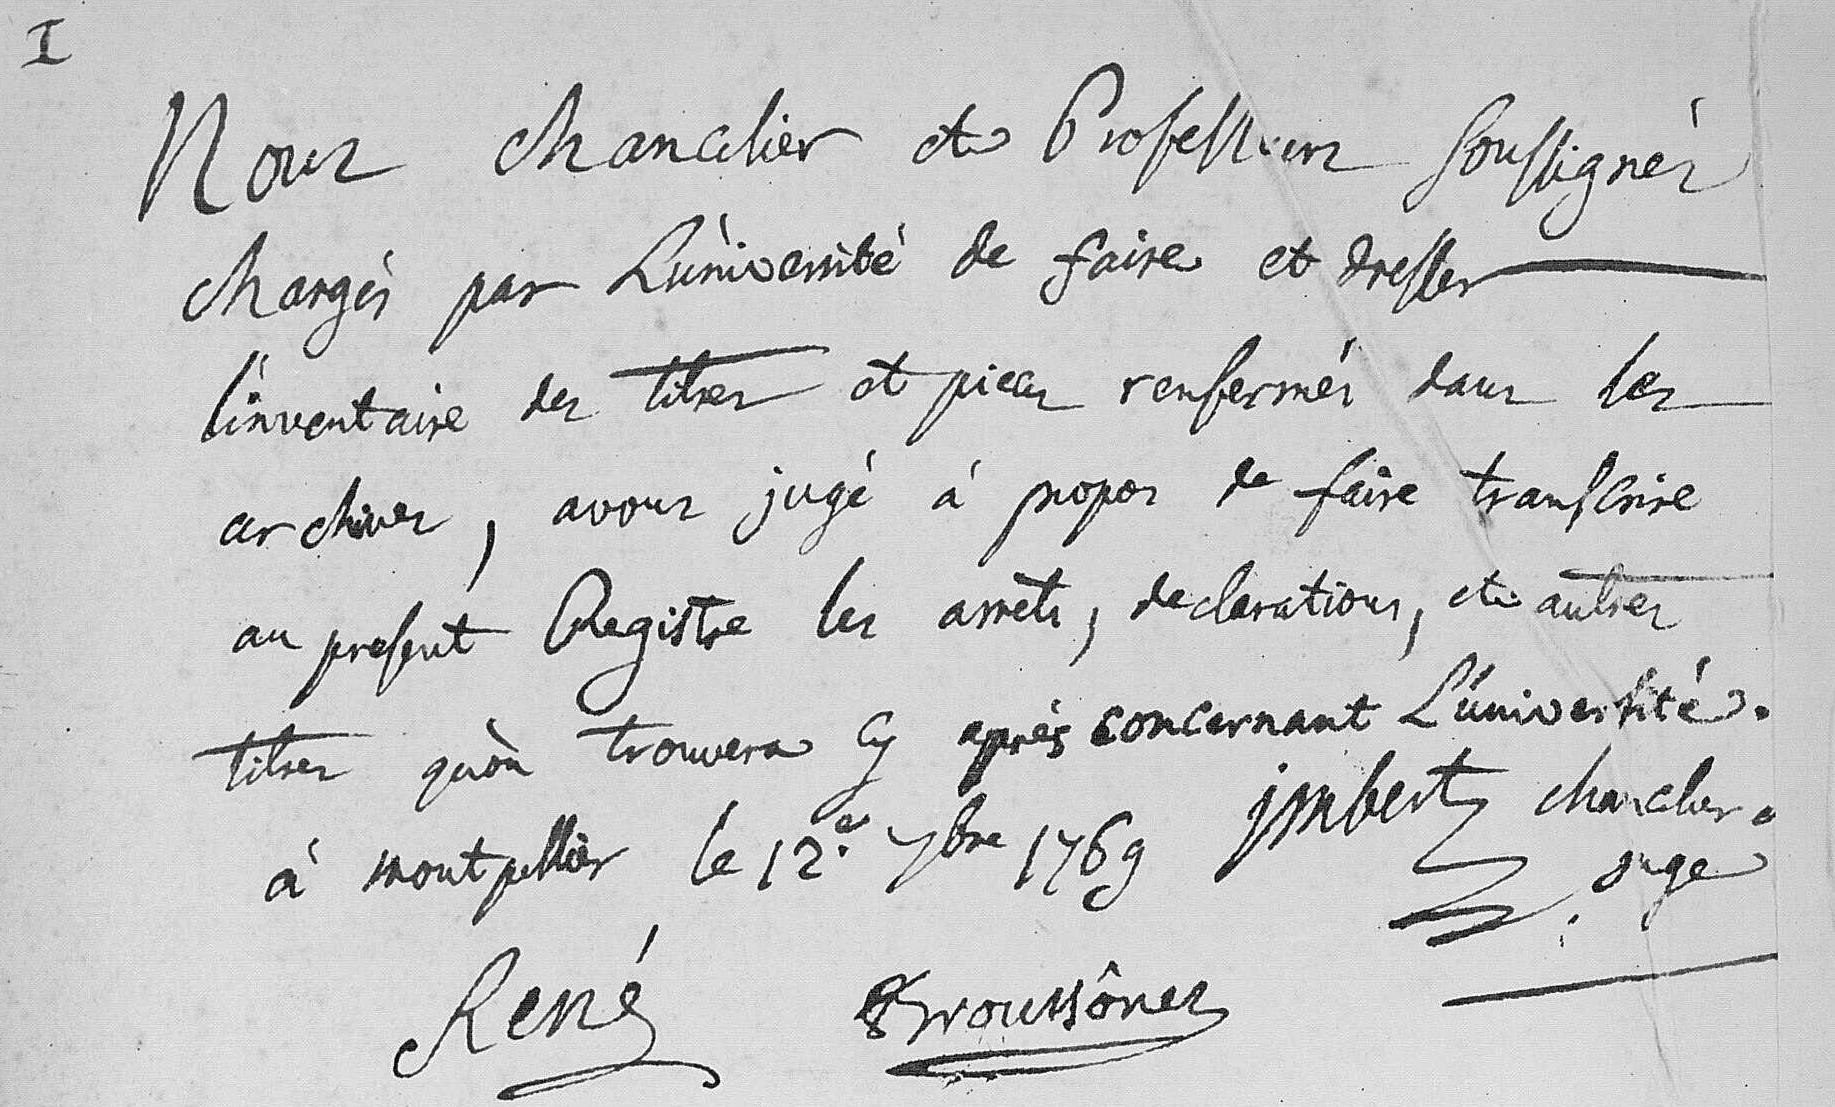
\includegraphics[
	width=\textwidth,
	height=0.78\textheight,
	keepaspectratio
	]{images/S3_f1.jpg}
	\caption[Ouverture du registre des \emph{Arrêts et Déclarations}, 12 septembre 1769]
	{Déclaration liminaire relative à la transcription des arrêts, déclarations et autres titres concernant l'Université, 12 septembre 1769, fol.~1, registre des \emph{Arrêts et Déclarations}, Montpellier, Archives historiques de la Faculté de médecine, S~3. Numérisation : Clara Martin.}
	\label{fig:s3-f1}
\end{figure}

\begin{figure}[p]
	\centering
	
	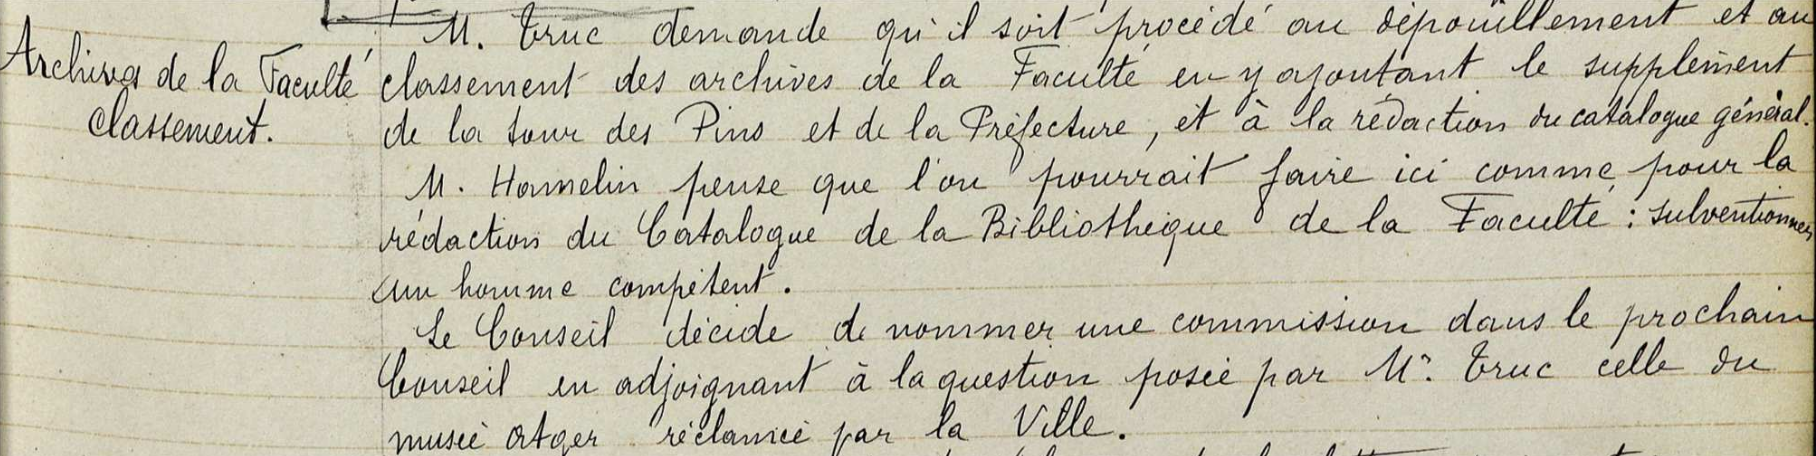
\includegraphics[
	width=\textwidth,
	height=0.30\textheight,
	keepaspectratio
	]{images/1MED51_calmette.png}
	\caption[Décision de classer les archives de la Faculté, 24 juillet 1902]
	{Délibération du conseil de faculté du 24 juillet 1902 décidant du classement des archives, Montpellier, Archives historiques de la Faculté de médecine, 1~MED~51. Numérisation : Sophie Dikoff.}
	\label{fig:1med51-calmette}
	
	\vspace{5em}
	
	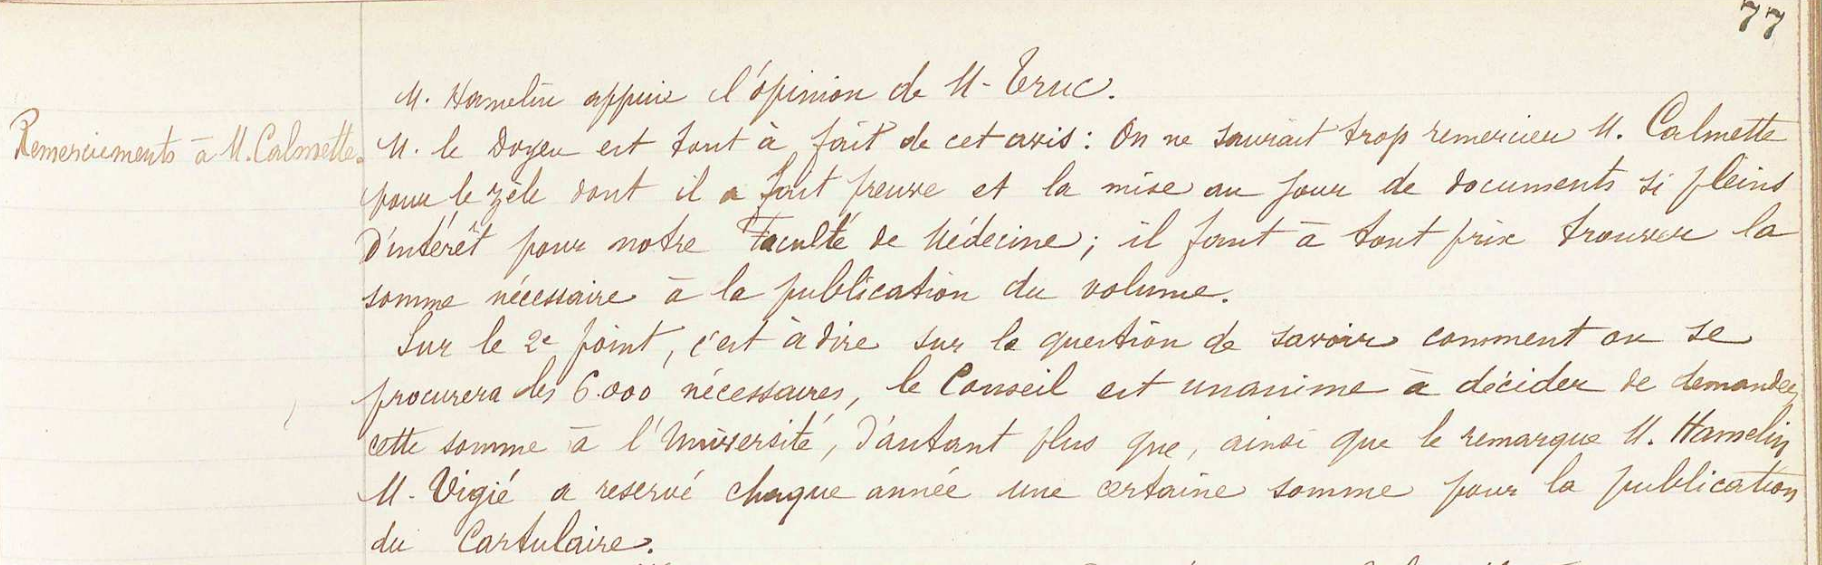
\includegraphics[
	width=\textwidth,
	height=0.30\textheight,
	keepaspectratio
	]{images/1MED52_calmette.png}
	\caption[Remerciements à Joseph Calmette et publication du \emph{Cartulaire}, 9 novembre 1907]
	{Délibération du conseil de faculté du 9 novembre 1907 remerciant Joseph Calmette et décidant de la publication du \emph{Cartulaire}, Montpellier, Archives historiques de la Faculté de médecine, 1~MED~52. Numérisation : Sophie Dikoff.}
	\label{fig:1med52-calmette}
\end{figure}

\chapter{Organisation de la Direction de la culture scientifique et du patrimoine historique}
\label{annexe:dcSPH}

\begin{landscape}
	\begin{figure}[p]
		\centering
		
		\rotatebox{180}{%
			\begin{minipage}{\linewidth}
				\centering
				
				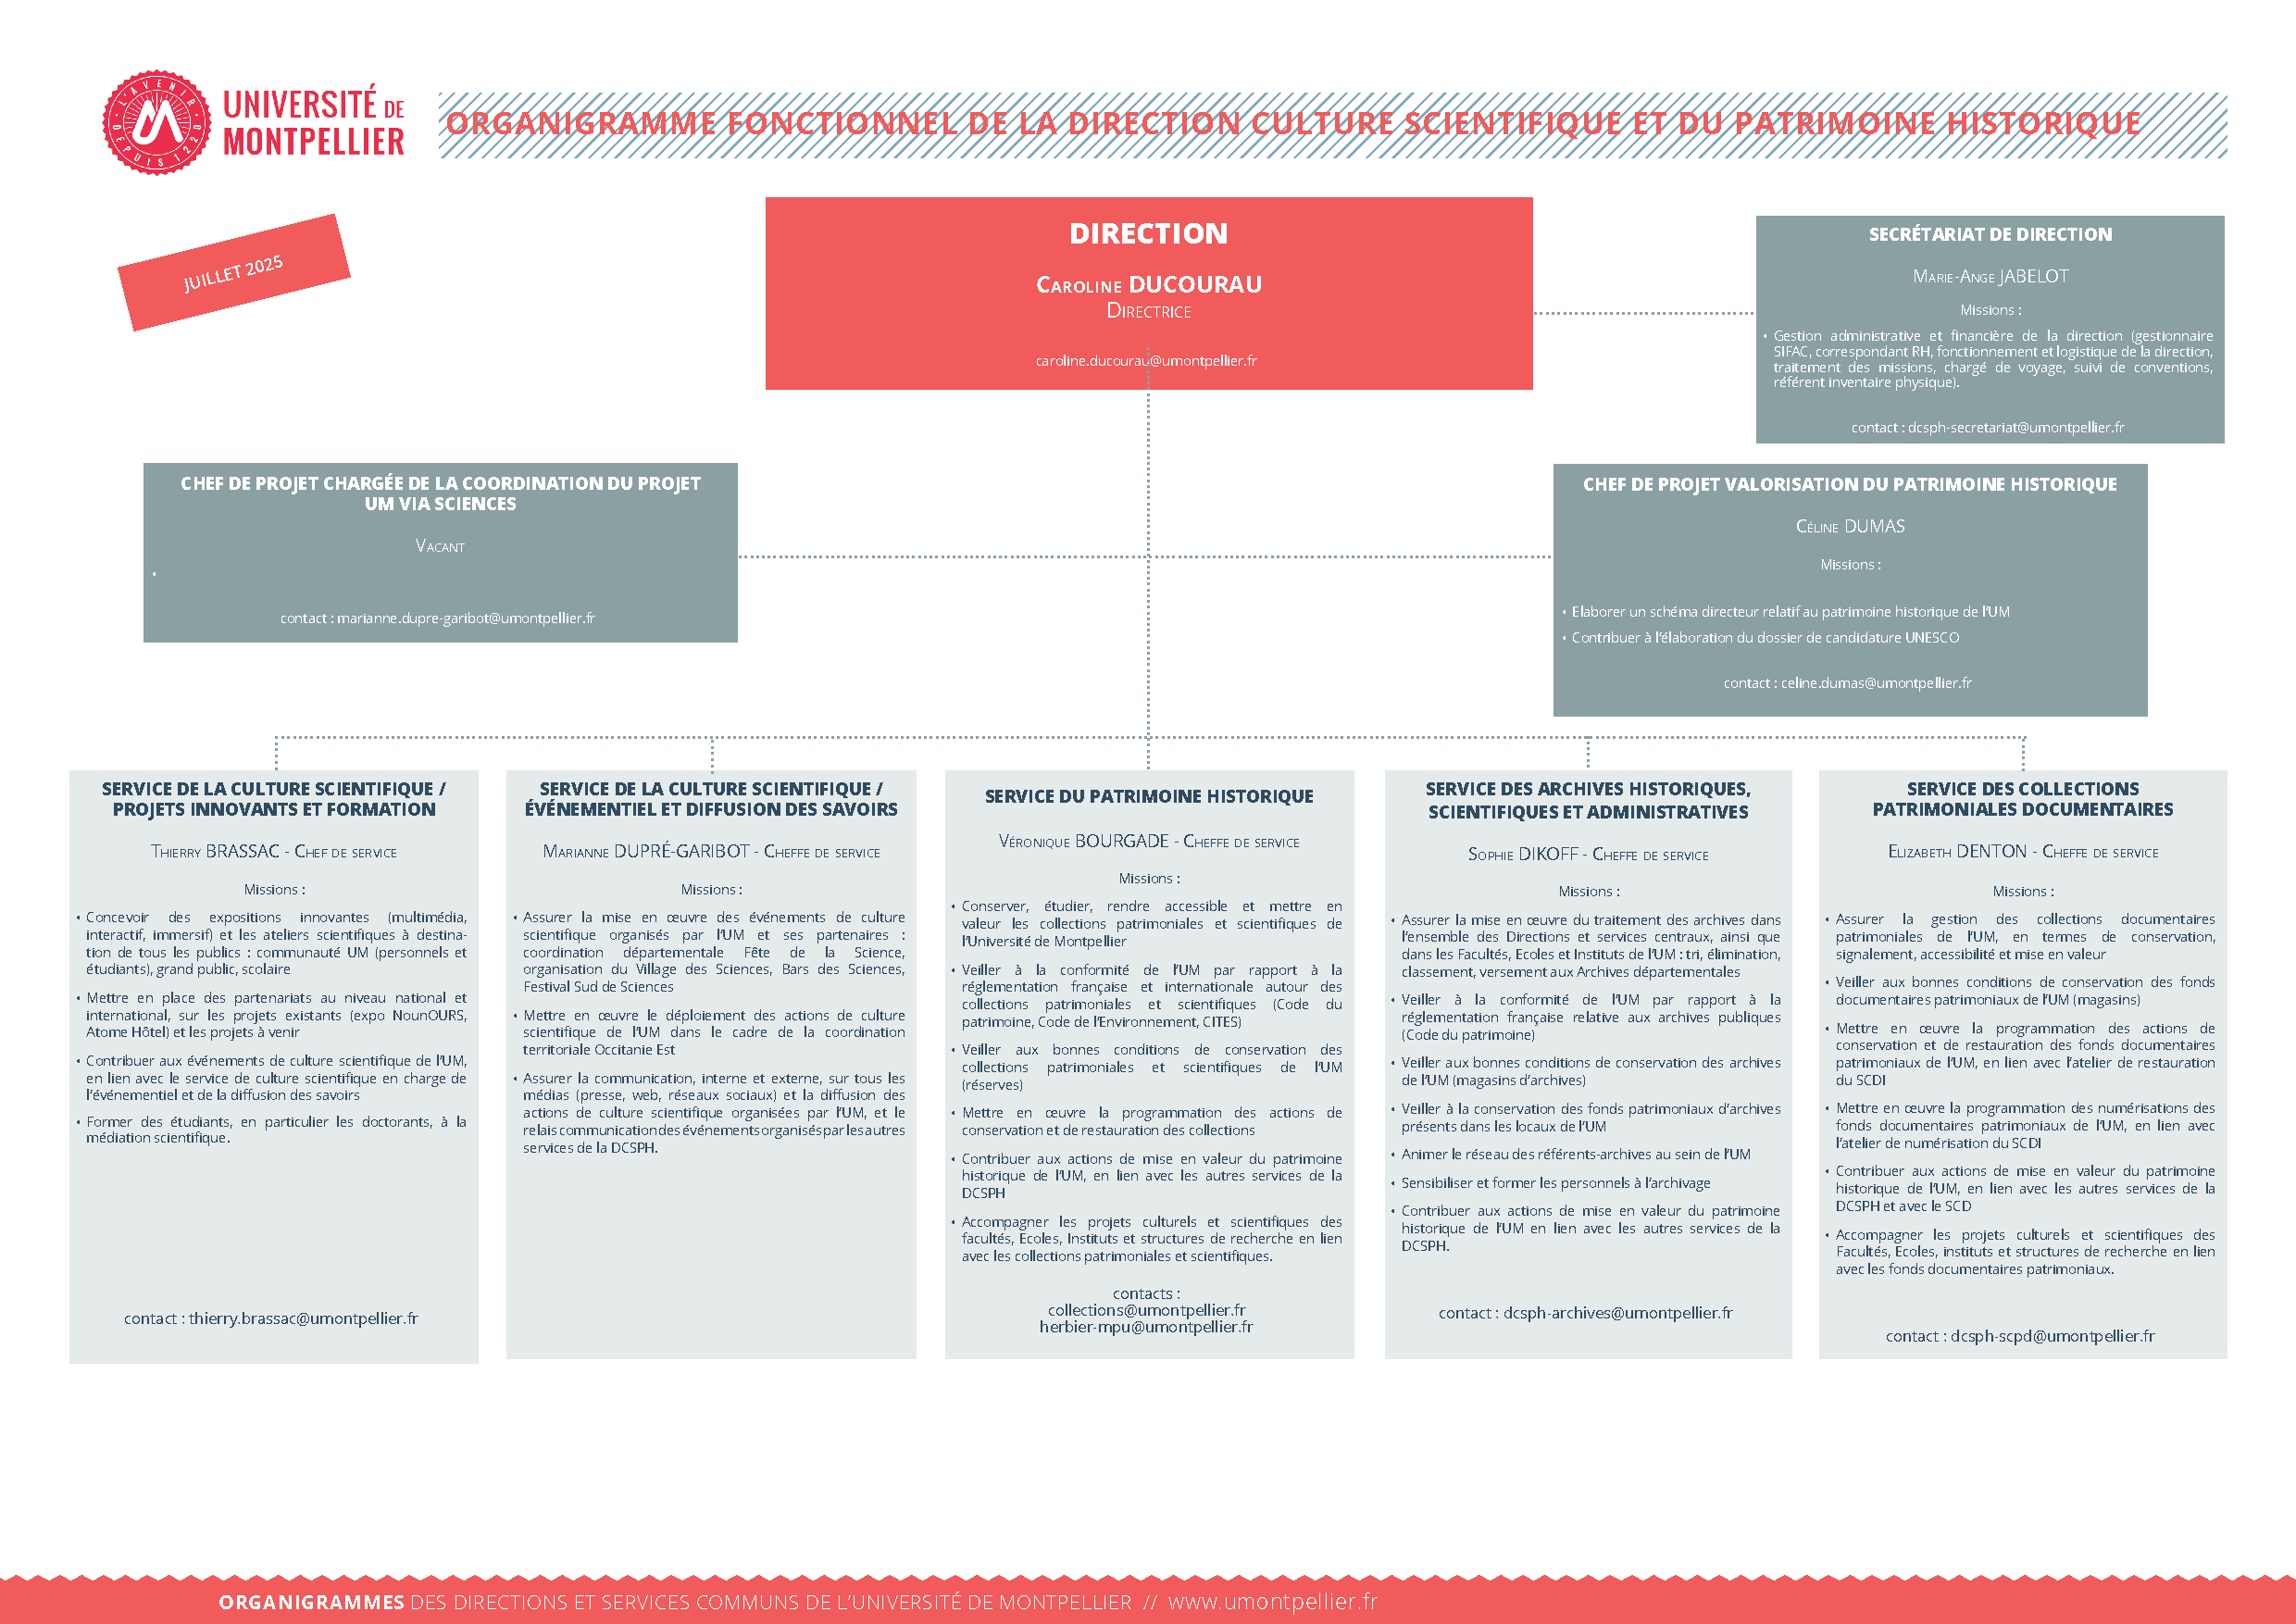
\includegraphics[
				page=1,
				width=1.08\linewidth,
				height=0.92\textheight,
				keepaspectratio
				]{images/DCSPH.pdf}
				
				\captionof{figure}
				[Organisation de la Direction de la culture scientifique et du patrimoine historique]
				{Organisation de la Direction de la culture scientifique et du patrimoine historique de l'Université de Montpellier, juillet 2025.}
				
				\label{fig:dcSPH-2025}
				
			\end{minipage}%
		}
		
	\end{figure}
\end{landscape}
